
%卒業論文用雛形
%\documentclass[a4j,12pt,oneside,openany]{jsbook}
% 英語なら以下を使う.
\documentclass[a4j,12pt,oneside,openany,english,dvipdfmx]{jsbook}

\usepackage{amsfonts,amsmath,amssymb}
\usepackage{bm}
\usepackage{float}
\usepackage[dvipdfmx]{graphicx}
\usepackage{color}
%\usepackage[dvipdfmx]{hyperref}
\usepackage{algorithm}
\usepackage{algorithmic}
%\usepackage{txfonts}
%\usepackage{ascmac, here}
\usepackage{listings}
\usepackage{color}
%\usepackage{url}
\usepackage{comment}

%jsbook を report っぽくするスタイルファイル
\usepackage{book2report}
%定理,補題,系,例題,証明などや英語用の定義がされています.
%自分なりにいじってください.
\usepackage{thesis}
% 具体的には以下のように定義されています.
% 英語の定理環境
%  \newtheorem{theorem}{Theorem}[chapter]
%  \newtheorem{lemma}{Lemma}[chapter]
%  \newtheorem{proposition}{Proposition}[chapter]
%  \newtheorem{corollary}{Corollary}[chapter]
%  \newtheorem{definition}{Definition}[chapter]
%  \newtheorem{example}{Example}[chapter]
%  \newtheorem{proof}{Proof}
% 日本語の定理環境
%  \newtheorem{theorem}{定理}[chapter]
%  \newtheorem{lemma}{補題}[chapter]
%  \newtheorem{proposition}{命題}[chapter]
%  \newtheorem{corollary}{系}[chapter]
%  \newtheorem{definition}{定義}[chapter]
%  \newtheorem{example}{例}[chapter]
%  \newtheorem{proof}{証明}
% 証明には番号をつけず,最後は Box で終わります.

\allowdisplaybreaks[1]

\newcommand{\mysps}{\ensuremath{[\![s^{\otimes}]\!]}_s}
\newcommand{\myspq}{\ensuremath{[\![s^{\otimes}]\!]}_q}
\newcommand{\myspds}{\ensuremath{[\![s^{\otimes \prime}]\!]}_s}
\newcommand{\myspdq}{\ensuremath{[\![s^{\otimes \prime}]\!]}_q}
\newcommand{\argmax}{\mathop{\rm arg~max}\limits}
\newcommand{\argmin}{\mathop{\rm arg~min}\limits}

\newtheorem{notations}{Notations}
\renewcommand{\thenotations}{\unskip}

% 英語で,見出しのフォントが気に入らなかったら
\renewcommand{\headfont}{\bfseries}

%ページ数が少ないときはここを大きくしてごまかそう!!効果絶大!!
\renewcommand{\baselinestretch}{1.1}

\begin{document}
%%%%%%%%%%%% 題目 %%%%%%%%%%%%%%%%%%%%%%%%%%%%%%%%%%%%%%%%%%%%%%%%%%%%%%%
%%%%%%%%%%%% ここも適当に変えてもいいと思う %%%%%%%%%%%%%%%%%%%%%%%%%%%%%%%%%
\thispagestyle{empty}
\begin{center}
\vspace*{5mm}
{\Huge {\bf 特 \hspace{12pt} 別 \hspace{12pt} 研 \hspace{12pt} 究 \hspace{12pt} 報 \hspace{12pt} 告}}\\
\vspace{2cm}
{\Large 題\hspace{8mm}目}\\
\vspace{1cm}
\underline{\Large{ Reinforcement Learning based Controller synthesis}} \\
\vspace{0.5cm}
\underline{\Large{ for Linear Temporal Logic Specifications }} \\
\vspace{0.5cm}
\underline{\Large{Using Limit-Deterministic Generalized B\"{u}chi Automata}} \\
\vspace{12mm}
{\large 指 導 教 員}\\
\vspace{6mm}
\underline{\Large 潮 俊光 教授}\\
 \\
%\underline{\Large Associate Professor Joe Smith}\\
\vspace{8mm}
{\large 報 告 者}\\
\vspace{6mm}
\underline{\Large 大浦 稜平}\\
\vspace{10mm}
{\Large 令和2年2月吉日}\\
\vspace{14mm}
{\Large 大阪大学基礎工学部システム科学科\\知能システム学コース}\\
\end{center}
\clearpage
\setcounter{page}{0}
\pagenumbering{roman}

%%%%%%%%%%%% 概要 %%%%%%%%%%%%%%%%%%%%%%%%%%%%%%%%%%%%%%%%%%%%%%%%%%%%
\begin{abstract}
  In this thesis, we propose a novel reinforcement learning method for the synthesis of a controller satisfying a control specification described by a linear temporal logic formula and apply the proposed method to supervisory control. We assume that the controlled system is modeled by a Markov decision process (MDP).
We transform the specification to a limit-deterministic generalized B\"{u}chi automaton (LDGBA) with several accepting sets that accepts all infinite sequences satisfying the formula.
The LDGBA is augmented so that it explicitly records the previous visits to accepting sets.
We take a product of the augmented LDGBA and the MDP, based on which we define a reward function. The agent gets rewards whenever state transitions are in an accepting set that has not been visited for a certain number of steps and the value function is maximized when all accepting sets are visited infinitely often.
Consequently, sparsity of rewards is relaxed and optimal circulations among the accepting sets are learned. We show that the proposed method can learn an optimal policy when the discount factor is sufficiently close to one.

\end{abstract}


%%%%%%%%%%%% 目次 %%%%%%%%%%%%%%%%%%%%%%%%%%%%%%%%%%%%%%%%%%%%%%%%%%%%
\clearpage
\tableofcontents
\clearpage
\setcounter{page}{0}
\pagenumbering{arabic}

%%%%%%%%%%%% 1章 %%%%%%%%%%%%%%%%%%%%%%%%%%%%%%%%%%%%%%%%%%%%%%%%%%%
\chapter{Introduction}

Temporal logic has been developed in computer engineering as a useful formalism of formal specifications  \cite{BK2008,Clarke2018}.
A merit of temporal logics is its resemblance to natural languages and it has been widely used in several other areas of engineering. Especially, a complicated mission or task in computer-controlled systems such as robots can be described by a temporal logic specification precisely and many synthesis algorithms of a controller or a planner that satisfies the specification have been proposed \cite{KB2008,Gazit2009,WTM2012a,SU2018}.
Linear temporal logic (LTL) is often used as a specification language because of its rich expressiveness.  It can explain many important $\omega$-regular properties such as liveness, safety, and persistence \cite{BK2008}.
It is known that the LTL specification is converted into an $\omega$-automaton such as a nondeterministic B\"{u}chi automaton and a deterministic Rabin automaton \cite{BK2008,Belta2017}.
In the synthesis of a control policy for the LTL specification,  we model a controlled system by a transition system that abstracts its dynamics, construct a product automaton of the transition system and the $\omega$-automaton corresponding to the LTL specification, and compute a winning strategy of a game over the product automaton \cite{Belta2017}.

Because of inherent stochasticity of controlled systems, we often use a Markov decision process (MDP) as a finite-state abstraction of the controlled systems \cite{Puterman}.
In the case where the probabilities are unknown a priori, we have two approaches to the synthesis of the control policy. One is robust control where we assume that state transition probabilities are in uncertainty sets \cite{WTM2012} while the other is learning using samples \cite{Sadigh2014}.

Reinforcement learning (RL) is a useful approach to learning an optimal policy from sample behaviors of the controlled system \cite{Sutton}.
In RL, we use a reward function that assigns a reward to each transition in the behaviors and evaluate a control policy by the return that is an expected (discounted) sum of the rewards along the behaviors.
Thus, to apply RL to the synthesis of a control policy for the LTL specification, it is an important issue how to introduce the reward function, which depends on the acceptance condition of an $\omega$-automaton converted from the LTL specification.
A reward function based on the acceptance condition of a Rabin automaton was proposed in \cite{Sadigh2014}. It was applied to a control problem where the controller optimizes a given control cost under the LTL constraint \cite{HU2015}.

Recently, a limit-deterministic B\"{u}chi automaton (LDBA) or generalized one (LDGBA) is paid much attention to as an $\omega$-automaton corresponding to the LTL specification \cite{SEJK2016}.
The RL-based approaches to the synthesis of a control policy using LDBAs have been proposed in \cite{HAK2019,Hahn2019,HKAKPL2019,BWZP2019}.
In \cite{Hahn2019,BWZP2019}, they use an LDBA. However, when constructing a B\"{u}chi automaton (BA) from a generalized B\"{u}chi automaton (GBA), the order of visits to accepting sets of the BA is fixed. The construction causes the sparsity of the reward based on the acceptance condition of a BA.
On the other hand, to deal with the acceptance condition of an LDGBA that accepts behaviors visiting all accepting sets infinitely often, the accepting frontier function was introduced in \cite{HAK2019,HKAKPL2019}. The reward function is defined based on the function.
However, the function is memoryless, that is, it does not provide the information of accepting sets that have been visited, which is important to improve learning performance.
In this letter, we propose a novel method to augment an LDGBA converted from a given LTL formula.
Then, we define a reward function based on the acceptance condition of the product MDP of the augmented LDGBA and the controlled system.
% based on the acceptance condition of the augmented automaton, embedded in the product MDP, which enables us to
As a result, we can improve the sparsity of rewards and expand the class of policies that satisfy the LTL specification compared to \cite{HAK2019}.

The rest of this thesis is organized as follows. Chapter 2 reviews Markov decision processes, reinforcement learning, linear temporal logic, and automata. Chapter 3 proposed a novel reinforcement learning based method for the synthesis of control policies. Chapter 4 proposed a novel reinforcement learning based supervisor synthesis with the method introduced in Chapter 3. Chapter 5 concludes the results and future works.


\begin{notations}
  For sets $A$ and $B$, $AB$ denotes their concatenation. $A^{\omega}$ denotes the infinite concatenation of the set $A$ and $A^{\ast}$ denotes the finite one. $\mathbb{N}_0$ is the set of nonnegative integers. $\mathbb{R}_{\geq 0}$ is the set of nonnegative real numbers.
\end{notations}

%%%%%%%%%%%% 2nd Chapter %%%%%%%%%%%%%%%%%%%%%%%%%%%%%%%%%%%%%%%%%%%%%%%%%%%
\chapter{Preliminaries}

\section{Markov Decision Processes}

We define a controlled system as a labeled Markov decision process.

\begin{definition}[Labeled Markov Decision Process]
  A (labeled) Markov decision process (MDP) is a tuple $M$ = $(S, A, P, s_{init}, AP, L)$, where S is a finite set of states, $A$ is a finite set of actions, $P:S \times S \times A \rightarrow [0,1]$ is a transition probability function, $s_{init} \in S$ is the initial state, $AP$ is a finite set of atomic propositions, and $L : S \times A \times S\ \rightarrow\ 2^{AP}$ is a labeling function that assigns a set of atomic propositions to each transition. Let $\mathcal{A}(s) = \{ a \in A ; \exists s^{\prime} \in S \text{ s.t. } P(s^{\prime} | s,a) \neq 0 \}$. Note that $\sum_{s' \in S} P(s'|s,a) = 1$ holds for any state $s \in S$ and action $a \in \mathcal{A}(s)$.

  In the MDP $M$, an infinite path starting from a state $s_0 \in S$ is defined as a sequence $\rho\ =\ s_0a_0s_1 \ldots\ \in S (A S)^{\omega}$ such that $P(s_{i+1}|s_i, a_i) > 0$ for any $ i \in \mathbb{N}_0$. A finite path is a finite sequence in $S (A S)^{\ast}$. In addition, we sometimes represent $\rho$ as $\rho_{init}$ to emphasize that $\rho$ starts from $s_0 = s_{init}$.
  For a path $\rho\ =\ s_0a_0s_1 \ldots$, we define the corresponding labeled path $L(\rho)\ =\ L(s_0,a_0,s_1)L(s_1,a_1,s_2) \ldots \in (2^{AP})^{\omega}$. $InfPath^{M}\ ( \text{resp., }FinPath^{M})$ is defined as the set of infinite (resp., finite) paths starting from $s_0=s_{init}$ in the MDP $M$. For each finite path $\rho$, $last(\rho)$ denotes its last state.
\label{MDP}
\end{definition}

\begin{definition}[Policy]
  A policy on an MDP $M$ is defined as a mapping $\pi:FinPath^{M} \times \mathcal{A}(last(\rho)) \rightarrow [0,1]$. A policy $\pi$ is a {\it positional} policy if for any $ \rho \in FinPath^{M}$ and any $ a \in \mathcal{A}(last(\rho))$, it holds that $\pi(\rho, a)=\pi(last(\rho),a)$ and there exists $ a' \in \mathcal{A}(last(\rho))$ such that
  \begin{align*}
    \pi(\rho, a) =
    \left\{
    \begin{aligned}
      1 &   & &\text{if}\ a=a',\\
      0 &   & &\text{otherwise}.
    \end{aligned}
    \right.
  \end{align*}
\end{definition}

Let $InfPath^{M}_{\pi}$ (resp., $FinPath^{M}_{\pi}$) be the set of infinite (resp., finite) paths starting from $s_0=s_{init}$ in the MDP $M$ under a policy $\pi$. The behavior of an MDP $M$ under a policy $\pi$ is defined on a probability space $(InfPath^{M}_{\pi}, \mathcal{F}_{InfPath^{M}_{\pi}}, Pr^{M}_{\pi})$. % over the set of infinite paths $InfPath^{M}_{\pi}$ on the MDP $M$ with the policy $\pi$.

\begin{definition}[Markov chain]
  A Markov chain induced by an MDP $M$ with a positional policy $\pi$ is a tuple $MC_{\pi} = (S_{\pi},P_{\pi},s_0,AP,L)$, where $S_{\pi} = S$, $P_{\pi}(s'|s) = P(s'|s,a)$ for $s, s^{\prime} \in S$ and $a \in \mathcal{A}(s)$ such that $\pi(s,a) = 1$.
  The state set $S_{\pi}$ of $MC_{\pi}$ can be represented as a disjoint union of a set of transient states $T_{\pi}$ and closed irreducible sets of recurrent states $R^j_{\pi}$ with $j \in \{ 1, \ldots ,h \}$, as $ S_{\pi} = T_{\pi} \sqcup R^1_{\pi} \sqcup \ldots \sqcup R^h_{\pi} $ \cite{ESS}.
  In the following, we say a ``recurrent class'' instead of a ``closed irreducible set of recurrent states'' for simplicity.
\end{definition}

In an MDP $M$, we define a reward function $\mathcal{R}:S \times A \times S \rightarrow \mathbb{R}$, where $\mathbb{R}$ is the set of real numbers. The function denotes the immediate scalar bounded reward received after the agent performs an action $a$ at a state $s$ and reaches a next state $s'$ as a result.

\section{Reinforcement Learning}

Reinforcement learning is the theoretical framework to find a policy maximizing or minimizing an objective function through the iterative interactions between the learner referred to the agent and the controlled system referred to the environment. The interaction is that the agent takes an action on the environment and the environment returns a observation such as a immediate reward or next state. In this section, since we use model-free method in this thesis, we refer the model-free reinforcement learning, which find a policy maximizing or minimizing an objective function without explicit estimations for the environment.

\subsection{Objective functions and an Optimal policy}

\begin{definition}[Expected discounted reward for MDPs]
  For a policy $\pi$ on an MDP $M$, any state $s \in S$, and a reward function $\mathcal{R}$, we define the expected discounted reward as
  \begin{align*}
    V^{\pi}(s)= \mathbb{E}^{\pi}[\sum_{n=0}^{\infty}\gamma^n \mathcal{R}(S_n, A_n, S_{n+1})|S_0 = s],
  \end{align*}
where $\mathbb{E}^{\pi}$ denotes the expected value given that the agent follows the policy $\pi$ from the state $s$ and $\gamma \in [0,1)$ is a discount factor. Intuitively, the magnitude of the discount factor $\gamma$ determines how much we consider rewards received in the future. The function $V^{\pi}(s)$ is often referred to as a state-value function under the policy $\pi$. For any state-action pair $(s,a) \in S \times A$, we define an action-value function $Q^{\pi}(s,a)$ under the policy $\pi$ as follows.
  \begin{align*}
    Q^{\pi}(s,a)= \mathbb{E}^{\pi}[\sum_{n=0}^{\infty}\gamma^n \mathcal{R}(S_n, A_n, S_{n+1})|&S_0 = s, A_0 = a].
  \end{align*}

  We have the following recursively equation for the state-value function and the action-value function.

  \begin{align}
    V^{\pi}(s) = & \mathbb{E}^{\pi}[\sum_{n=0}^{\infty}\gamma^n \mathcal{R}(S_n, A_n, S_{n+1})|S_0 = s] \nonumber \\
     = & \sum_{a \in \mathcal{A}(s)} \pi(s,a) \sum_{s^{\prime} \in S} P(s^{\prime}|s,a) \mathbb{E}^{\pi}[\sum_{n=0}^{\infty}\gamma^n \mathcal{R}(S_n, A_n, S_{n+1})|S_0 = s, A_0 = a, S_1 = s^{\prime}] \nonumber \\
     = & \sum_{a \in \mathcal{A}(s)} \pi(s,a) \sum_{s^{\prime} \in S} P(s^{\prime}|s,a) \{ \mathcal{R}(s, a, s^{\prime}) + \gamma \mathbb{E}^{\pi}[\sum_{n=0}^{\infty}\gamma^n \mathcal{R}(S_n, A_n, S_{n+1})|S_1 = s^{\prime}] \} \nonumber \\
    = & \sum_{a \in \mathcal{A}(s)} \pi(s,a) \sum_{s^{\prime} \in S} P(s^{\prime}|s,a) \{ \mathcal{R}(s, a, s^{\prime}) + \gamma V^{\pi}(s^{\prime}) \},
    \label{V_pi}
  \end{align}
\end{definition}

by the definition of the action-value function, it holds that

\begin{align}
  Q^{\pi}(s,a) = & \max_{a \in \mathcal{A}(s)}V^{\pi}(s) \nonumber \\
               = & \sum_{s^{\prime} \in S} P(s^{\prime}|s,a) \{ \mathcal{R}(s, a, s^{\prime}) + \gamma V^{\pi}(s^{\prime}) \} \nonumber \\
               = & \sum_{s^{\prime} \in S} P(s^{\prime}|s,a) \{ \mathcal{R}(s, a, s^{\prime}) + \gamma \sum_{a^{\prime} \in \mathcal{A}(s^{\prime})} \pi(s^{\prime}, a^{\prime}) Q^{\pi}(s^{\prime},a^{\prime}) \}.
 \label{Q_pi}
\end{align}
 The above equations are called the {\it Bellman equation}.

\begin{definition}[Optimal policy]
  For any state $s \in S$, a policy $\pi^{\ast}$ is optimal if
  \begin{align*}
    \pi^{\ast} \in \argmax_{\pi \in \Pi^{pos}} V^{\pi}(s),
  \end{align*}
where $\Pi^{pos}$ is the set of positional policies over the state set $S$.

We have the following {\it Bellman optimality functions} by the definition of optimal policies.

\begin{align}
  V^{\ast}(s) := & V^{\pi^{\ast}}(s) \nonumber \\
               = & \max_{\pi \in \Pi^{pos}} V^{\pi}(s) \nonumber \\
                    = & \max_{\pi \in \Pi^{pos}} \sum_{a \in \mathcal{A}(s)} \pi(s,a) \sum_{s^{\prime} \in S} P(s^{\prime}|s,a) \{ \mathcal{R}(s, a, s^{\prime}) + \gamma V^{\pi}(s^{\prime}) \} \nonumber \\
                    = & \max_{a \in \mathcal{A}(s)} [ \sum_{s^{\prime} \in S} P(s^{\prime}|s,a) \{ \mathcal{R}(s, a, s^{\prime}) + \gamma V^{\pi^{\ast}}(s^{\prime}) \} ],
\label{opt_V}
\end{align}

\begin{align}
  Q^{\ast}(s,a) := & Q^{\pi^{\ast}}(s,a) \nonumber \\
                = & \max_{\pi \in \Pi^{pos}} Q^{\pi}(s,a) \nonumber \\
                      = & \max_{\pi \in \Pi^{pos}} \sum_{s^{\prime} \in S} P(s^{\prime}|s,a) \{ \mathcal{R}(s, a, s^{\prime}) + \gamma \sum_{a^{\prime} \in \mathcal{A}(s^{\prime})} \pi(s^{\prime}, a^{\prime}) Q^{\pi}(s^{\prime},a^{\prime}) \} \nonumber \\
                      = & \sum_{s^{\prime} \in S} P(s^{\prime}|s,a) \{ \mathcal{R}(s, a, s^{\prime}) + \gamma \max_{\pi \in \Pi^{pos}} \sum_{a^{\prime} \in \mathcal{A}(s^{\prime})} \pi(s^{\prime}, a^{\prime}) Q^{\pi}(s^{\prime},a^{\prime}) \} \nonumber \\
                      = & \sum_{s^{\prime} \in S} P(s^{\prime}|s,a) \{ \mathcal{R}(s, a, s^{\prime}) + \gamma \max_{a \in \mathcal{A}(s^{\prime})} Q^{\pi}(s^{\prime},a^{\prime}) \}.
\label{opt_Q}
\end{align}
\label{opt_pol}
\end{definition}

We call $V^{\ast}$ and $Q^{\ast}$ the optimal state-value function and the optimal action-value function, respectively. $V^{\ast}(s)$ represents $Q^{\ast}(s,a)$ with an optimal action at the first step. Therefor, for any state $s \in S$, we have

\begin{align*}
  V^{\ast}(s) = \max_{a \in \mathcal{A}(s)} Q^{\ast}(s,a)
\end{align*}

In words, the set of optimal policies under $V^{\ast}$ and the set of optimal polisies under $Q^{\ast}$ are the same.

If we know the full and accurate information of an MDP such as the transition probability or the reward function, we can obtain an optimal policy by solving Eqs. \ref{opt_V} or \ref{opt_Q} directly. we usually use {\it Dynamic Programming} by solving recursively equation such as Eqs \ref{opt_V} or \ref{opt_Q}. To find $V^{\pi}$ or $Q^{\pi}$ for a policy $\pi$ by solving Eqs. \ref{V_pi} or \ref{Q_pi} is referred to {\it Policy Evaluation}. For any state $s \in S$ or any state-action pair $(s,a) \in S \times A$, to update the policy $\pi$ to increase the value of $V^{\pi}(s)$ or $Q^{\pi}(s,a)$ is referred to {\it Policy Improvement}. The method that finds an optimal policy by updating optimal value function repeatedly in accordance with Eqs. \ref{opt_V} ar \ref{opt_Q} is referred to {\it Value Iteration}. The method that finds an optimal policy by repeating policy evaluation and policy improvement alternately is referred to {\it Policy Iteration}.

\subsection{Temporal Difference Learning}

If the MDP $M$ is unknown, we can not use Dynamic programming such as value iteration or policy iteration to obtain an optimal policy. In the case that the MDP $M$ is unknown, we often use   reinforcement learning to find an optimal policy instead of dynamic programming.

Temporal difference learning (TD-learning) is the basic method of model-free reinforcement learning. The method does not require the prior knowledge about the environment and utilize a raw experience by one step. Unlike dynamic programing, we update a value function using the experience in an on-line and incremental manner as follows.

\begin{align}
  \hat{V}^{\pi_k}(s_k) \leftarrow \hat{V}^{\pi_k}(s_k) + \alpha_k \{ r_{k+1} + \hat{V}^{\pi_k}(s_{k+1}) - \hat{V}^{\pi_k}(s_k) \},
\end{align}
where $\pi_k$, $s_k$, and $\alpha_k$ are the policy, the state, and the learning ratio at the time step $k$, respectively, and $r_{k+1} = \mathcal{R}(s_k, a_k, s_{k+1})$. Note that $\alpha_k \in [0,1]$ for any $k \in \mathbb{N}_0$. The quantity in the curly bracket in the right hand side is called {\it TD-error}

\begin{align}
  \Delta_k = r_{k+1} + \hat{V}^{\pi_k}(s_{k+1}) - \hat{V}^{\pi_k}(s_k).
\end{align}

TD-error represents the difference between the current estimated value function and the better estimated value function of a current state based on an actual experience, namely $r_{k+1} + \hat{V}^{\pi_k}(s_{k+1})$. Intuitively, as the value function repeatedly is updated, the errors is gradually reduced. Hence, the magnitude of the learning ratio $\alpha_k$ describes how much we influence the better estimated value at the current state based on the most recent experience on the current estimated value at the current state.

TD-learning methods for an action-value function are classified as two main learning methods that are referred to {\it Q-learning} and {\it SARSA}.
In Q-learning, we do not use the actual action at the next state to update the current estimated state-action value at the current state-action pair. Instead we use the optimal action at the next state to update the estimated state-action value function. That is, the way of update the estimated state-action value function $\hat{Q}^{\pi_k}(s_k, a_k)$ at time step $k$ is as follows

\begin{align}
  \hat{Q}^{\pi_k}(s_k,a_k) \leftarrow \hat{Q}^{\pi_k}(s_k,a_k) + \alpha_k \{ r_{k+1} + \max_{a^{\prime} \in \mathcal{A}(s_{k+1})} \hat{Q}^{\pi_k}(s_{k+1}, a^{\prime}) - \hat{Q}^{\pi_k}(s_k,a_k) \}.
\end{align}

On the other hand, in SARSA, we use the actual action at the next state to update the current estimated state-action value function. That is,

\begin{align}
  \hat{Q}^{\pi_k}(s_k,a_k) \leftarrow \hat{Q}^{\pi_k}(s_k,a_k) + \alpha_k \{ r_{k+1} + \hat{Q}^{\pi_k}(s_{k+1}, a_{k+1}) - \hat{Q}^{\pi_k}(s_k,a_k) \}.
\end{align}

\section{Linear Temporal Logic and Automata}

In our proposed method, we use linear temporal logic (LTL) formulas to describe various constraints or properties and to systematically assign corresponding rewards.
%For some complicated constraints, it is hard to assign such a corresponding reward function and to find a policy satisfying an LTL formula by the conventional reward assignments.
LTL formulas are constructed from a set of atomic propositions, Boolean operators, and temporal operators. We use the standard notations for the Boolean operators: $\top$ (true), $\neg$ (negation), and $\land$ (conjunction).
LTL formulas over a set of atomic propositions $AP$ are recursively defined as
\begin{align*}
  \varphi ::=\top\ |\ \alpha \in AP\ |\ \varphi_1 \land \varphi_2\ |\ \neg \varphi\ |\ \text{{\bf X}} \varphi\ |\ \varphi_1 \text{{\bf U}} \varphi_2,
\end{align*}
where $\varphi$, $\varphi_1$, and $\varphi_2$ are LTL formulas.
Additional Boolean operators are defined as $\perp := \neg \top $, $\varphi_1 \lor \varphi_2 := \neg(\neg \varphi_1 \land \neg \varphi)$, and $\varphi_1 \Rightarrow \varphi_2 := \neg \varphi_1 \lor \varphi_2$.
The operators {\bf X} and {\bf U} are called ``next" and ``until", respectively.
Using the operator {\bf U}, we define two temporal operators: (1) {\it eventually}, $\text{{\bf F}} \varphi := \top \text{{\bf U}} \varphi $ and (2) {\it always}, $\text{{\bf G}} \varphi := \neg \text{{\bf F}} \neg \varphi$.

Let $ M $ be an MDP.
For an infinite path $\rho = s_0a_0s_1 \ldots $ of $ M $ with $ s_0 \in S $, let $\rho[i]$ be the $i$-th state of $\rho$ i.e., $\rho[i]=s_i$ and let $\rho[i:]$ be the $i$-th suffix $\rho[i:]=s_ia_is_{i+1} \ldots $. We define the $i$-th state and $i$-th suffix of the infinite path for a DES in the same way.
% let $\rho[:i]$ be the $i$-th prefix $\rho[:i]=s_0 \ldots s_{i-1}a_{i-1}s_i$,and let $\rho[i:j]$ be the finite sequence $\rho[i:j]=s_ia_is_{i+1} \ldots s_{j-1}a_{j-1}s_{j}$.
\begin{definition}[LTL semantics]
	For an LTL formula $\varphi$, an MDP $M$, and an infinite path $\rho = s_0a_0s_1 \ldots$ of $ M $ with $ s_0 \in S $, the satisfaction relation $M,\rho \models \varphi$ is recursively defined as follows.
	\begin{alignat}{2}
	& M, \rho \models \top,\nonumber \\
	& M, \rho \models \alpha \in AP &&\Leftrightarrow \alpha \in L(s_0,a_0,s_1),\nonumber \\
	& M, \rho \models \varphi_1 \land \varphi_2 &&\Leftrightarrow M, \rho \models \varphi_1 \land M, \rho \models \varphi_2,\nonumber \\
	& M, \rho \models \neg \varphi &&\Leftrightarrow M, \rho \not\models \varphi,\nonumber \\
	& M, \rho \models \text{{\bf X}}\varphi &&\Leftrightarrow M, \rho[1:] \models \varphi,\nonumber \\
	& M, \rho \models \varphi_1 \text{{\bf U}} \varphi_2 &&\Leftrightarrow \exists j \geq 0, \ M, \rho[j:] \models \varphi_2 \land \forall i, 0\leq i < j, \ M, \rho[i:] \models \varphi_1.\nonumber
	\end{alignat}
The next operator {\bf X} requires that $\varphi$ is satisfied by the next state suffix of $\rho$. The until operator {\bf U} requires that $\varphi_1$ holds true until $\varphi_2$ becomes true over the path $\rho$. For the path in a DES, we define the LTL semantics in the same way.
Using the operator {\bf U} we can define two temporal operators: (1) {\it eventually}, $\text{{\bf F}} \varphi := \top \text{{\bf U}} \varphi $ and (2) {\it always}, $\text{{\bf G}} \varphi := \neg \text{{\bf F}} \neg \varphi$.
In the following, we write $ \rho \models \varphi $ for simplicity without referring to MDP $ M $ and DES $D$.
%For an LTL formula $ \varphi $ over $ AP $,
%we denote by $ \mathcal{L}(\varphi) \subset (2^{AP})^\omega $ the set of all words that satisfy $\varphi$.


For any policy $\pi$, the probability of all paths starting from $s_{init}$ on the MDP $M$ that satisfy an LTL formula $\varphi$ under the policy $\pi$, or the satisfaction probability is defined as follows.
\begin{align*}
Pr^{M}_{\pi}(s_{init} \! \models \varphi) := Pr^{M}_{\pi}(\{ \rho_{init} \! \in \! InfPath^{M}_{\pi} ; \rho_{init} \! \models \varphi \}).
\end{align*}
We say that an LTL formula $\varphi$ is satisfied by a positional policy $\pi$ (resp., a supervisor $SV$) if
\begin{align*}
Pr^{M}_{\pi}(s_{init} \models \varphi) > 0.
\end{align*}



\label{def5}
\end{definition}

Any LTL formula $\varphi$ can be converted into various automata, namely finite state machines that recognize %$\mathcal{L}$($\varphi$).
all words satisfying $\varphi$.
 We define a generalized B\"{u}chi automaton at the beginning, and then introduce a limit-deterministic B\"{u}chi automaton \cite{HKAKPL2019}.

 \begin{definition}[Transition-based generalized B\"{u}chi automata]
   A transition-based generalized B\"{u}chi automaton (tGBA) is a tuple $B = (X,\ x_{init},\ \Sigma,\ \delta,\ \mathcal{F})$, where $X$ is a finite set of states, $x_{init} \in X$ is the initial state, $\Sigma$ is an input alphabet including $\varepsilon$, $\delta \subset  X\times \Sigma \times X$ is a set of transitions, and $\mathcal{F} = \{F_1,\ldots,F_n\}$ is an acceptance condition, where for each $ j \in \{1,\ldots,n\}$, $F_j \subset \delta$ is a set of accepting transitions and called an accepting set. We refer to a tGBA with one accepting set as a tBA.

   Let $\Sigma^{\omega}$ be the set of all infinite words over $\Sigma$ and let an infinite run be an infinite sequence $r = x_0\sigma_0x_1 \ldots \in X (\Sigma X)^{\omega}$ where $(x_i, \sigma_{i}, x_{i+1}) \in \delta\ $ for any $ i\in \mathbb{N}_0$. An infinite word $w = \sigma_0\sigma_1 \ldots \in \Sigma^{\omega}$ is accepted by $B_{\varphi}$ if and only if there exists an infinite run $r = x_0 \sigma_0 x_1 \ldots$ starting from $x_0 = x_{init}$ such that $inf(r) \cap F_j \neq \emptyset\ $ for each $F_j \in \mathcal{F}$, where $inf(r)$ is the set of transitions that occur infinitely often in the run $r$.
 \end{definition}

\begin{definition}[Sink state]
A sink state in state set $X$ of an augmented tLDBA $\bar{B}_{\varphi} = (\bar{X}, \bar{x}_{init},\bar{\Sigma},\bar{\delta},\bar{\mathcal{F}})$ is defined as a state such that there exist no accepting transition of $\bar{B}_{\varphi}$ that is accessible from the state. We denote the set of sink states as $Sink Set$.
\end{definition}

\begin{definition}[Limit-deterministic generalized B\"{u}chi automata]
  A transition-based limit-deterministic generalized B\"{u}chi automaton (tLDGBA) is a tGBA $B = (X, x_{init},\Sigma,\delta,\mathcal{F})$ such that $X$ is partitioned into two disjoint sets $X_{initial}$ and $X_{final}$ such that
  \begin{itemize}
    \item $F_j \subset X_{final} \times \Sigma \times X_{final}$, $\forall j \in \{ 1,...,n \}$,
    %\item $| \{ (x, \sigma, x^{\prime}) \! \in \! \delta; x^{\prime} \! \in \! X_{initial} \} | \! \leq \! 1$, $\forall x \! \in \! X_{initial}, \forall \sigma \! \in \! \Sigma$,
    \item $| \{ (x, \sigma, x^{\prime}) \in \delta; x^{\prime} \in X_{final} \} | \! \leq \! 1$, $\forall x \! \in \! X_{final}, \forall \sigma \! \in \! \Sigma$,
    \item $| \{ (x, \sigma, x^{\prime}) \in \delta; x^{\prime} \in X_{initial} \} |$=0, $\forall x \! \in \! X_{final}, \forall \sigma \! \in \! \Sigma$.
    \item there are $\varepsilon$-transitions into $X_{final}$ from $X_{initial}$.
\end{itemize}
\end{definition}
  An $\varepsilon$-transition enables the tLDGBA to change its state with no input. Then, the $\varepsilon$-transitions reflect the single ``guess" from $X_{initial}$ to $X_{final}$. Note that by the construction in \cite{SEJK2016}, the transitions in each part are deterministic except for $\varepsilon$-transitions into $X_{final}$ from $X_{intial}$.
It is known that, for any LTL formula $ \varphi $, there exists a tLDGBA that accepts all words satisfying $\varphi$ \cite{SEJK2016}. We refer to a tLDGBA with one accepting set as a tLDBA.
%in $ \mathcal{L}(\varphi) $ \cite{SEJK2016}.
In particular, we represent a tLDGBA recognizing an LTL formula $\varphi$ as $B_{\varphi}$, whose input alphabet is given by $ \Sigma = 2^{AP} \cup \{ \varepsilon \} $.


%%%%%%%%%%%% 3rd Chapter %%%%%%%%%%%%%%%%%%%%%%%%%%%%%%%%%%%%%%%%%%%%%%%%%%%
\chapter{Reinforcement learning based control policy synthesis for LTL specifications}

\section{Augmentation of tLDGBAs and Synthesis Method}

We introduce an automaton augmented with binary vectors. The automaton can explicitly represent whether transitions in each accepting set occur at least once, and ensure transitions in each accepting set occur infinitely often.

Let $V = \{ (v_1, \ldots ,v_n)^T\ ;\ v_i \in \{ 0,1 \},\ i \in \{ 1, \ldots ,n \} \}$ be a set of binary-valued vectors, and let $\bm{1}$ and $\bm{0}$ be the $n$-dimentional vectors with all elements 1 and 0, respectively.
In order to augment a tLDBA $B_{\varphi}$, we introduce three functions $visitf:\delta \rightarrow V$, $reset:V \rightarrow V$, and $Max:V\times V \rightarrow V$ as follows.
For any $e \in \delta$, $visitf(e) = (v_1, \ldots ,v_n)^T$, where %$ v_i = 1 $ if $ e \in F_i $ and $ v_i=0 $ otherwise.
\begin{align}
 v_i =
  \left\{
  \begin{aligned}
    1 &   & &\text{if}\ e\in F_i, \\
    0 &   & &\text{otherwise}.
  \end{aligned}
  \right. \nonumber
\end{align}
For any $v \in V$, %$ reset(v) = \bm{0} $ if $ v = \bm{1} $ and $ reset(v) = v $ otherwise.
\begin{align}
  &reset(v) =
  \left\{
  \begin{aligned}
    \bm{0} &   & &\text{if}\  v = \bm{1},\\
    v &   & &\text{otherwise}.
  \end{aligned}
  \right. \nonumber
\end{align}
For any $v,u \in V$, $Max(v,u) = (l_1,\ldots ,l_n)^T$, where $l_i = max\{v_i, u_i\} $ for any $i\in \{1, \ldots ,n\}$.

Each vector $v$ is called a memory vector and represents which accepting sets have been visited. The function $visitf$ returns a binary vector whose $i$-th element is 1 if and only if a transition in the accepting set $F_i$ occurs. The function $reset$ returns the zero vector $\bm{0}$ if at least one transition in each accepting set has occurred after the latest reset. Otherwise, it returns the input vector without change.

\begin{definition}[Augmented Automata]
   For a tLDGBA $B_{\varphi} = (X,x_{init},\Sigma,\delta,\mathcal{F})$, its augmented automaton is a tLDGBA $\bar{B}_{\varphi}$ = $(\bar{X},\bar{x}_{init},\bar{\Sigma},\bar{\delta},\bar{\mathcal{F}})$, where $\bar{X} = X\times V$, $\bar{x}_{init} = (x_{init}, \bm{0})$, $\bar{\Sigma} = \Sigma$, $\bar{\delta}$ is defined as $\bar{\delta}$ = $\{ ((x,v), \bar{\sigma}, (x^{\prime},v^{\prime})) \in \bar{X} \times \bar{\Sigma} \times \bar{X}\ ;\ (x,\bar{\sigma},x^{\prime}) \in \delta,\ v^{\prime} = reset(Max(v,visitf((x,\bar{\sigma},x^{\prime})))) \}$, and $\mathcal{\bar{F}} = \{ \bar{F_1}, \ldots ,\bar{F_n} \}$ is defined as $\bar{F_i} = \{ ((x,v), \bar{\sigma}, (x^{\prime},v^{\prime})) \in \bar{\delta}\ ;\ (x, \sigma, x^{\prime}) \in F_i,\ v_i = 0 \}$ for each $ i \in \{1,...,n\}$.
   \label{augment_def}
\end{definition}

%It is obvious by Definition \ref{augment_def} that a tLDGBA and its augmented automaton accept the same language.
We denote by $\mathcal{L}(B)$ the accepted language of a tLDGBA $B$, namely the set of all infinite words accepted by $B$.

\begin{proposition}
  Let $ B = (X,x_{init},\Sigma,\delta,\mathcal{F}) $ and $ \bar{B} = (\bar{X},\bar{x}_{init},\bar{\Sigma},\bar{\delta},\bar{\mathcal{F}}) $ be an arbitrary tLDGBA and its augmentation, respectively.
Then, we have $ \mathcal{L}(B) = \mathcal{L}(\bar{B}) $.
\label{prop3-1}
\end{proposition}
The proof of Proopsition \ref{prop3-1} is shown in Appendix A.

The augmented tLDGBA $\bar{B}_{\varphi}$ keeps track of previous visits to the accepting sets of $B_{\varphi}$.
Intuitively,
% for an input word $w$,
along a run of $\bar{B}_\varphi$,
a memory vector $v$ is reset to $\bm{0}$ when at least one transition in each accepting set of the original tLDGBA $B_{\varphi}$ has occurred.
% along the corresponding run of $B_{\varphi}$.

For example, shown in Figs.\ \ref{automaton} and \ref{automaton_aug} are a tLDGBA and its augmented automaton, respectively, associated with the following LTL formula.
\begin{align}
  \varphi = \text{{\bf GF}}a \land \text{{\bf GF}}b \land \text{{\bf G}}\neg c.
  \label{ltl}
\end{align}
The acceptance condition ${\mathcal F}$ of the tLDGBA is given by ${\mathcal F} = \{ F_1,F_2 \}$, where $F_1=\{ (x_0, \{ a \}, x_0),\ (x_0, \{ a,b \}, x_0) \}$ and $F_2 = \{ (x_0, \{ b \}, x_0),\ (x_0, \{ a,b \}, x_0) \}$.
Practically, states in a strongly connected component that contains no accepting transitions can be merged as shown in Fig.\ \ref{automaton_aug}.

\begin{figure}[htbp]
   \centering
%   \vspace{2mm}
%   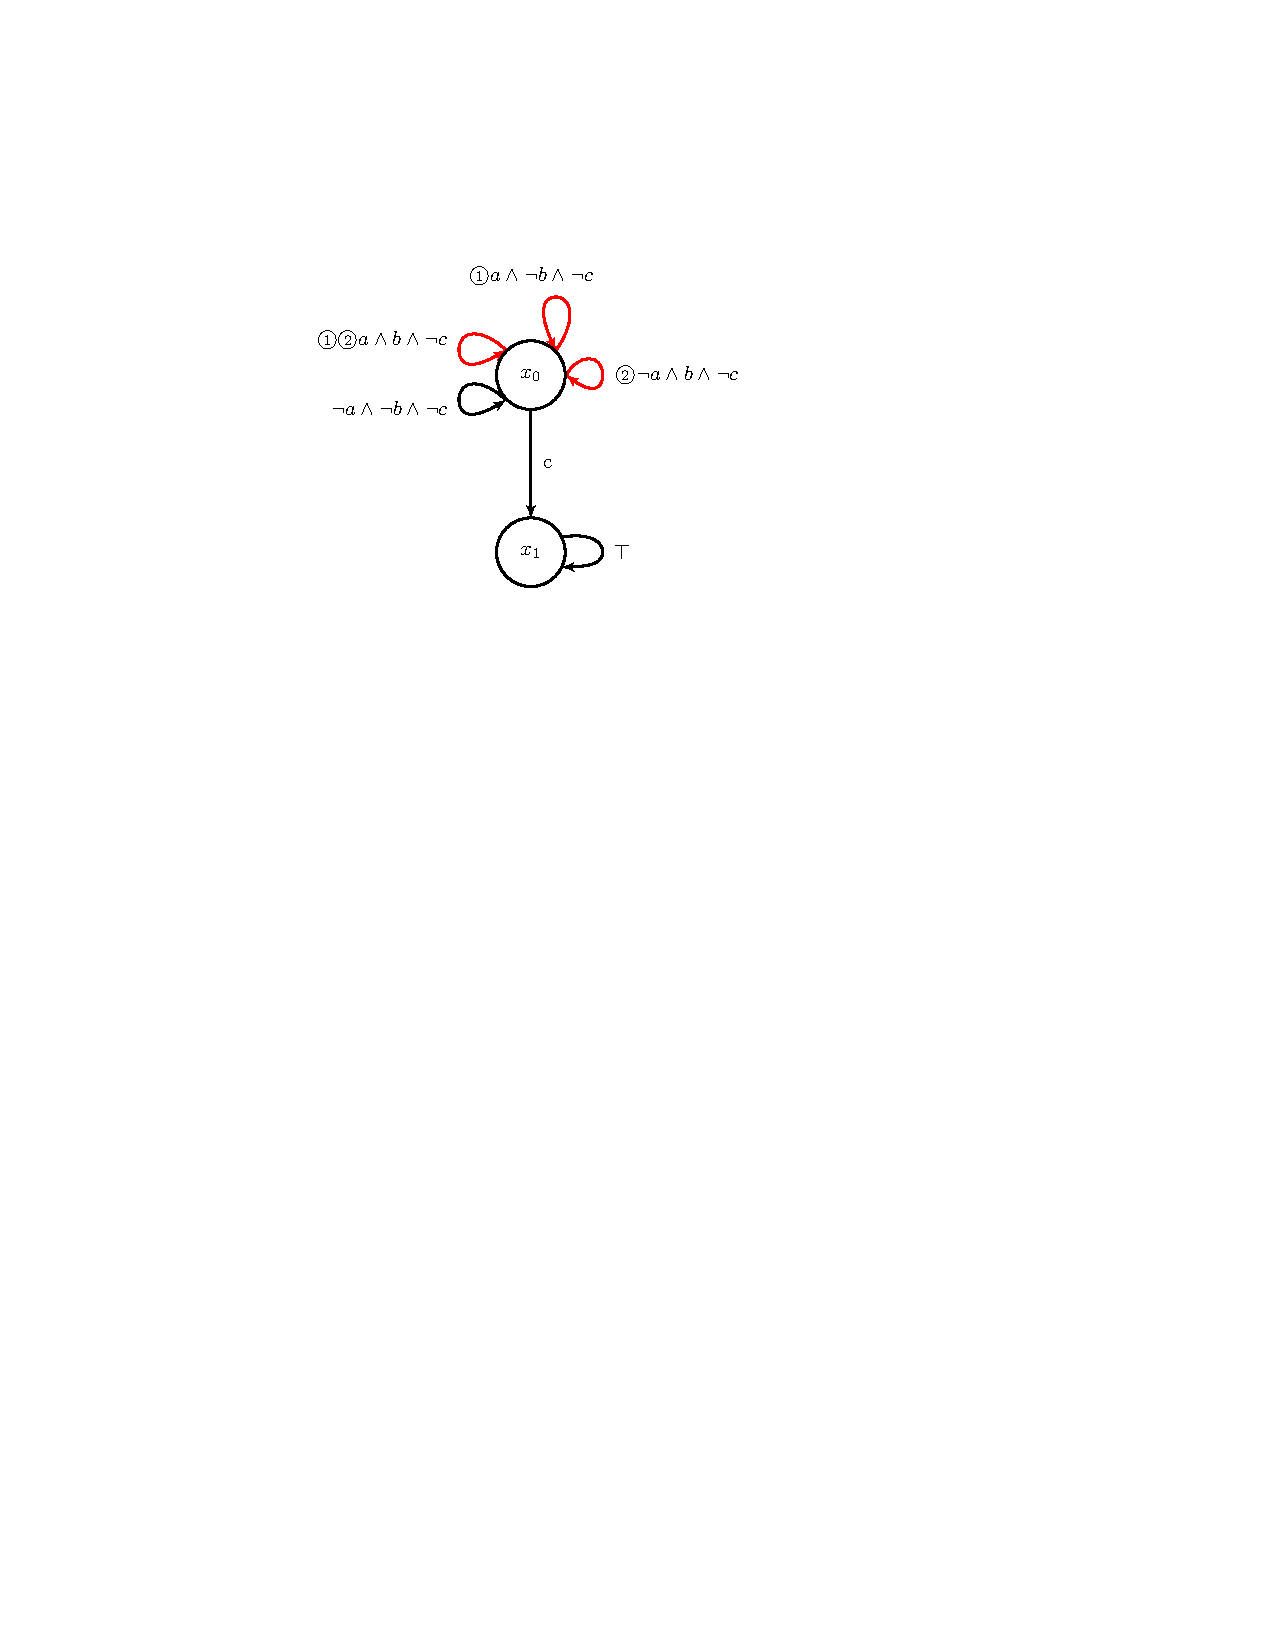
\includegraphics[bb=140 498 368 682,width=5cm]{automaton1.pdf}
   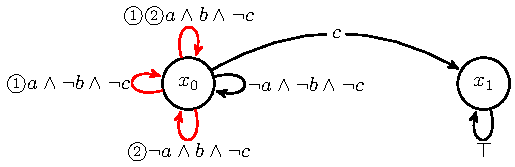
\includegraphics[bb=0 0 247 80,scale=0.8]{ldgba_original.pdf}
   \caption{The tLDGBA recognizing the LTL formula $\text{{\bf GF}}a \wedge \text{{\bf GF}}b \wedge \text{{\bf G}}\neg c$, where the initial state is $x_0$. Red arcs are accepting transitions that are numbered in accordance with the accepting sets they belong to.}
   % e.g., \textcircled{\scriptsize 1}$a \land \neg b \land \neg c$ means the transition labeled by it belongs to the accepting set $F_1$.}
   \label{automaton}
\end{figure}
\begin{figure}[htbp]
   \centering
%   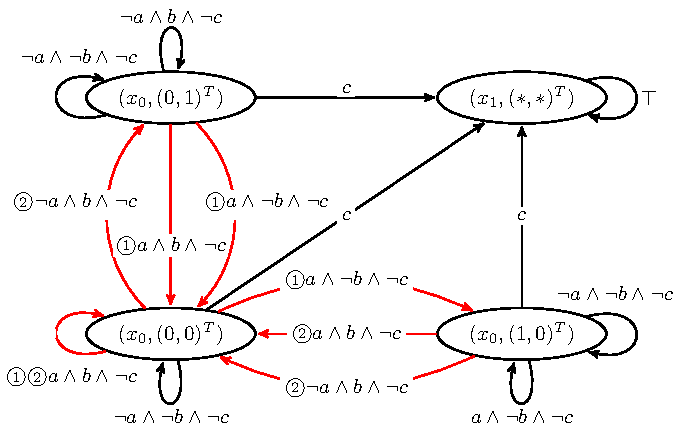
\includegraphics[bb=0 0 374 207,height=4cm, width=7cm]{ldgba.pdf}
   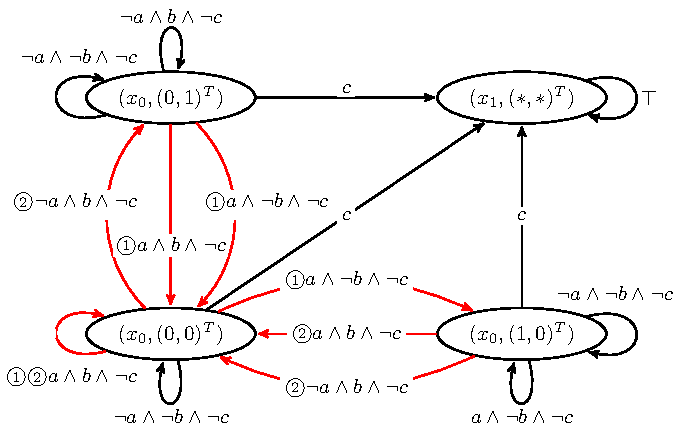
\includegraphics[bb=0 0 326 207,scale=0.8]{ldgba.pdf}
   \caption{The augmented automaton for the tLDGBA in Fig.~\ref{automaton} recognizing the LTL formula $\text{{\bf GF}}a \wedge \text{{\bf GF}}b \wedge \text{{\bf G}}\neg c$, where the initial state is $(x_0, (0,0)^T )$. Red arcs are accepting transitions that are numbered in accordance with the accepting sets they belong to. All states corresponding to $x_1$ are merged into $(x_1, (*,*)^T )$.}
   \label{automaton_aug}
\end{figure}

We modify the standard definition of a product MDP to deal with $\varepsilon$-transitions in the augmented automaton.
\begin{definition}[Product MDPs]
  Given an augmented tLDGBA $\bar{B}_{\varphi}$ and an MDP $M$, a tuple $M \otimes \bar{B}_{\varphi} = M^{\otimes} = (S^{\otimes}, A^{\otimes},s_{init}^{\otimes}, P^{\otimes}, \delta^{\otimes},$ $ {\mathcal F}^{\otimes})$ is a product MDP, where
  $S^{\otimes} = S \times \bar{X}$ is the finite set of states;
  $A^{\otimes}$  is the finite set of actions such that $A^{\otimes}=A \cup \{ \varepsilon_{\bar{x}^{\prime}} ; \exists \bar{x}^{\prime}\! \in \! X \text{ s.t. } (\bar{x},\varepsilon,\bar{x}^{\prime}) \in \bar{\delta} \}$, where $\varepsilon_{\bar{x}^{\prime}}$ is the action for the $\varepsilon$-transition to the state $\bar{x}^{\prime}\! \in\! \bar{X}$;
  $s_{init}^{\otimes} = (s_{init},\bar{x}_{init})$ is the initial state; $P^{\otimes} : S^{\otimes} \times S^{\otimes} \times A^{\otimes} \rightarrow [0,1]$ is the transition probability function defined as
%   $P^{\otimes}(s^{\otimes \prime} | s^{\otimes}, a) = P(s^{\prime} | s, a)$ if $ (\bar{x}, L((s,a,s^{\prime})), \bar{x}^{\prime}) \in \bar{\delta}$ and $ a \in \mathcal{A}(s)$, $P^{\otimes}(s^{\otimes \prime} | s^{\otimes}, a) = 1$ if $s\!=\!s^{\prime}, (\bar{x}, \varepsilon, \bar{x}^{\prime})\! \in \! \bar{\delta},$ and $ a=\varepsilon_{x^{\prime}}$, otherwise $P^{\otimes}(s^{\otimes \prime} | s^{\otimes}, a) = 0$
%   \begin{comment}
  \begin{align*}
    &P^{\otimes}(s^{\otimes \prime} | s^{\otimes}, a) \\ &=
    \left\{
    \begin{aligned}
      &P(s^{\prime} | s, a) &   &\text{if}\  (\bar{x}, L((s,a,s^{\prime})), \bar{x}^{\prime}) \in \bar{\delta}, a \in \mathcal{A}(s)\\
      &1 &   &\text{if}\ s=s^{\prime}, (\bar{x}, \varepsilon, \bar{x}^{\prime}) \in  \bar{\delta}, a=\varepsilon_{\bar{x}^{\prime}},\\
      &0 &   &\text{otherwise} ,
    \end{aligned}
    \right. \nonumber
  \end{align*}
% \end{comment}
  where $s^{\otimes}=(s,(x,v))$ and $s^{\otimes \prime}=(s^{\prime},(x^{\prime},v^{\prime}))$;
  $\delta^{\otimes} = \{ (s^{\otimes}, a, s^{\otimes \prime})\in S^{\otimes} \times A^{\otimes} \times S^{\otimes} ; P^{\otimes}(s^{\otimes \prime} | s^{\otimes}, a) > 0 \}$ is the set of transitions;
  and ${\mathcal F}^{\otimes} = \{ \bar{F}^{\otimes}_1, \ldots ,\bar{F}^{\otimes}_n \}$ is the acceptance condition, where $\bar{F}^{\otimes}_i = \{ ((s,\bar{x}), a, (s^{\prime}, \bar{x}^{\prime})) \in \delta^{\otimes} ; (\bar{x}, L(s,a,s^{\prime}), \bar{x}^{\prime}) \in \bar{F}_i \}$ for each $ i \in \{ 1, \ldots ,n \}$.
  \begin{comment}
   We have to modify the definition of product MDP to deal with $\varepsilon$-transitions in the original tLDBA $B_{\varphi}$. First, for all $\varepsilon$-transition from $x \in X$ to $x^{\prime} \in X$ of $B_{\varphi}$, we add the $\varepsilon_{x^{\prime}}$-action into the product MDP, namely $\mathcal{A}^{\otimes}(s^{\otimes}) = \mathcal{A}^{\otimes}(s^{\otimes}) \cup \{ \varepsilon_{x^{\prime}} ; s^{\otimes} = (s,(x,v)),\ s^{\otimes \prime} = (s,(x^{\prime}, v)),\ x,x^{\prime} \in X \}$. Second, the transition probability associated with the $\varepsilon_{x^{\prime}}$-action is defined as
  \begin{align}
    P^{\otimes}(s^{\otimes \prime} | s^{\otimes}, a) =
    \left\{
    \begin{aligned}
      &1 &   &\text{if}\ (s\!=\!s^{\prime})\! \land\! (v\!=\!v^{\prime})\! \land\! (x, \varepsilon_{x^{\prime}}, x^{\prime})\! \in \! \bar{\delta},\\
      &0 &   &\text{otherwise} ,
    \end{aligned}
    \right. \nonumber
  \end{align}
  where $s^{\otimes}=(s,(x,v))$ and $s^{\otimes}=(s^{\prime},(x^{\prime},v^{\prime}))$.
\end{comment}

\label{def9}
\end{definition}

\begin{definition}[Reward assignments]
  The reward function $\mathcal{R} :S^{\otimes} \times A^{\otimes} \times S^{\otimes} \rightarrow {\mathbb R}_{\geq 0}$ is defined as
  \begin{align}
    \mathcal{R}(s^{\otimes}, a, s^{\otimes \prime}) =
    \left\{
    \begin{aligned}
      &r_p \  \text{if}\ \exists i \in \! \{ 1, \ldots ,n \},\ (s^{\otimes}, a, s^{\otimes \prime}) \in \bar{F}^{\otimes}_i \!,\\
      &0   \ \ \text{otherwise},
    \end{aligned}
    \right. \nonumber
  \end{align}
  where $r_p$ is a positive value.
  \label{def10}
\end{definition}

%The reward assignments are based on the acceptance conditions of the product MDP.
Under the product MDP $M^{\otimes}$ and the reward function $\mathcal{R}$, which is based on the acceptance condition of $ M^\otimes $, we show that if there exists a positional policy $\pi$ satisfying the LTL specification $\varphi$, maximizing the expected discounted reward produces a policy satisfying $\varphi$.

For a Markov chain $MC^{\otimes}_{\pi}$ induced by a product MDP $M^{\otimes}$ with a positional policy $\pi$, let $S^{\otimes}_{\pi}= T^{\otimes}_{\pi} \cup R^{\otimes 1}_{\pi} \cup \ldots \cup R^{\otimes h}_{\pi}$ be the set of states in $MC^{\otimes}_{\pi}$, where $T^{\otimes}_{\pi}$ is the set of transient states and $R^{\otimes i}_{\pi}$ is the recurrent class for each $i \in \{ 1, \ldots ,h \}$, and let $R(MC^{\otimes}_{\pi})$ be the set of all recurrent classes in $MC^{\otimes}_{\pi}$. Let $\delta^{\otimes}_{\pi,i}$ be the set of transtions in a recurrent class $R^{\otimes i}_{\pi}$, namely $\delta^{\otimes}_{\pi,i} = \{ (s^{\otimes},a,s^{\otimes \prime}) \in \delta^{\otimes} ; s^{\otimes} \in R^{\otimes i}_{\pi},\ P^{\otimes}(s^{\otimes \prime}|s^{\otimes},a) > 0 \}$, and let $P^{\otimes}_{\pi}$ : $S^{\otimes}_{\pi} \times S^{\otimes}_{\pi} \rightarrow [0,1]$ be the transition probability under $\pi$.

\begin{lemma}
  For any policy $\pi$ and any recurrent class $R^{\otimes i}_{\pi}$ in the Markov chain $MC^{\otimes}_{\pi}$,
  $MC^{\otimes}_{\pi}$ satisfies one of the following conditions.
  \vspace{2mm}
  \begin{enumerate}
    \item $\delta^{\otimes}_{\pi,i} \cap \bar{F}^{\otimes}_j \neq \emptyset\ $, $ \forall j \in \{ 1, \ldots ,n \}$,
    \item $\delta^{\otimes}_{\pi,i} \cap \bar{F}^{\otimes}_j = \emptyset\ $, $ \forall j \in \{ 1, \ldots ,n \}$.
  \end{enumerate}
  \label{lemma3-1}
\end{lemma}
The proof of Lemma \ref{lemma3-1} is shown in Appendix A.

Lemma \ref{lemma3-1} implies that, for an LTL formula $\varphi$ if a path $\rho$ under a policy $\pi$ does not satisfy $\varphi$, then the agent obtains no reward in recurrent classes; otherwise there exists at least one recurrent class where the agent obtains rewards infinitely often.

\begin{theorem}
  Let $M^{\otimes}$ be the product MDP corresponding to an MDP $M$ and an LTL formula $\varphi$. If there exists a positional policy satisfying $\varphi$, then there exists a discount factor $\gamma^{\ast}$ such that any algorithm that maximizes the expected reward with $\gamma > \gamma^{\ast}$ will find a positional policy satisfying $\varphi$.
  \label{theorem3-1}
\end{theorem}
The proof of Theorem \ref{theorem3-1} is shown in Appendix A.

%\begin{theorem}
%  Let $M^{\otimes}$ be the product MDP corresponding to an MDP $M$ and an LTL formula $\varphi$. If there exists a positional policy $\pi$ such that $Pr^M_{\pi}(\rho_{init} \models \varphi) = 1$, then there exists a discount factor $\gamma^{\ast}$ such that any algorithm that maximizes the expected reward with $\gamma > \gamma^{\ast}$ will find a positional policy $\pi^{\prime}$ such that $Pr^M_{\pi^{\prime}}(\rho_{init} \models \varphi) = 1$.
%  \label{theorem3-2}
%\end{theorem}

We show the overall procedure of our proposed method in Algorithm \ref{syn_pol}. We employ Q-learning in Algorithm \ref{syn_pol}, but any algorithms maximizing the expected discounted reward can be applied to our proposed method.
\begin{algorithm}
 \caption{RL-based synthesis of control policy on the MDP with the augmented tLDBA.}
 \begin{algorithmic}[1]
 \renewcommand{\algorithmicrequire}{\textbf{Input:}}
 \renewcommand{\algorithmicensure}{\textbf{Output:}}
 \REQUIRE LTL formula $\varphi$ and MDP $M$
 \ENSURE  Optimal policy $\pi^{\ast}$ on the product MDP $M^{\otimes}$
 \STATE Translate $\varphi$ into tLDBA $B_{\varphi}$.
  \STATE Augment $B_{\varphi}$ to $\bar{B}_{\varphi}$.
  \STATE Construct the product MDP $M^{\otimes}$ of $M$ and $\bar{B}_{\varphi}$.
  \STATE Initialize $Q:S^{\otimes} \times A^{\otimes} \rightarrow \mathbb{R}_{\geq 0}$.
  \STATE Initialize episode length $T$.
  \WHILE {$Q$ is not converged}
  \STATE $s^{\otimes} \leftarrow (s_{init},(x_{init},\bm{0}))$.
  \FOR {$t = 1$ to $T$}
  \STATE Choose the action $a$ by a policy $\pi$.
  \STATE Observe the next state $s^{\otimes \prime}$.
  \STATE $Q(s^{\otimes},a) \leftarrow Q(s^{\otimes},a) + \alpha \{ \mathcal{R}(s^{\otimes},a,s^{\otimes \prime}) + \gamma \max_{a^{\prime}}Q(s^{\otimes \prime},a^{\prime}) - Q(s^{\otimes},a) \}$
  \STATE $s^{\otimes} \leftarrow s^{\otimes \prime}$
  \ENDFOR
  \ENDWHILE
 \end{algorithmic}
 \label{syn_pol}
\end{algorithm}

\section{Example}

\begin{figure}[tbp]
    \centering
    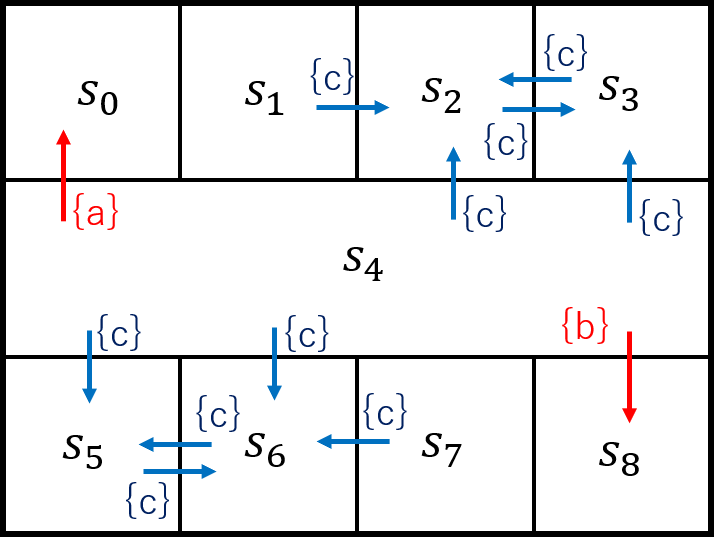
\includegraphics[bb=0 0 377 290,height=3.5cm,width=5cm]{MDP_corridor.png}
%    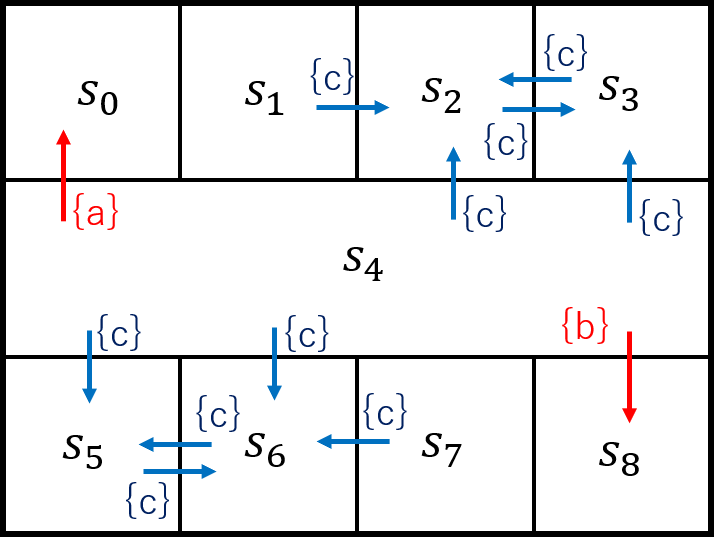
\includegraphics[height=4cm, width=6cm]{MDP_corridor.png}
    \caption{The environment consisting of eight rooms and one corridor. Red arcs are the transitions that we want to occur infinitely often, while blue arcs are the transitions that we never want to occur. $s_7$ is the initial state.}
    \label{Grid1}
\end{figure}

\begin{comment}
\begin{figure}[htbp]
   \centering
   \vspace{2mm}
%   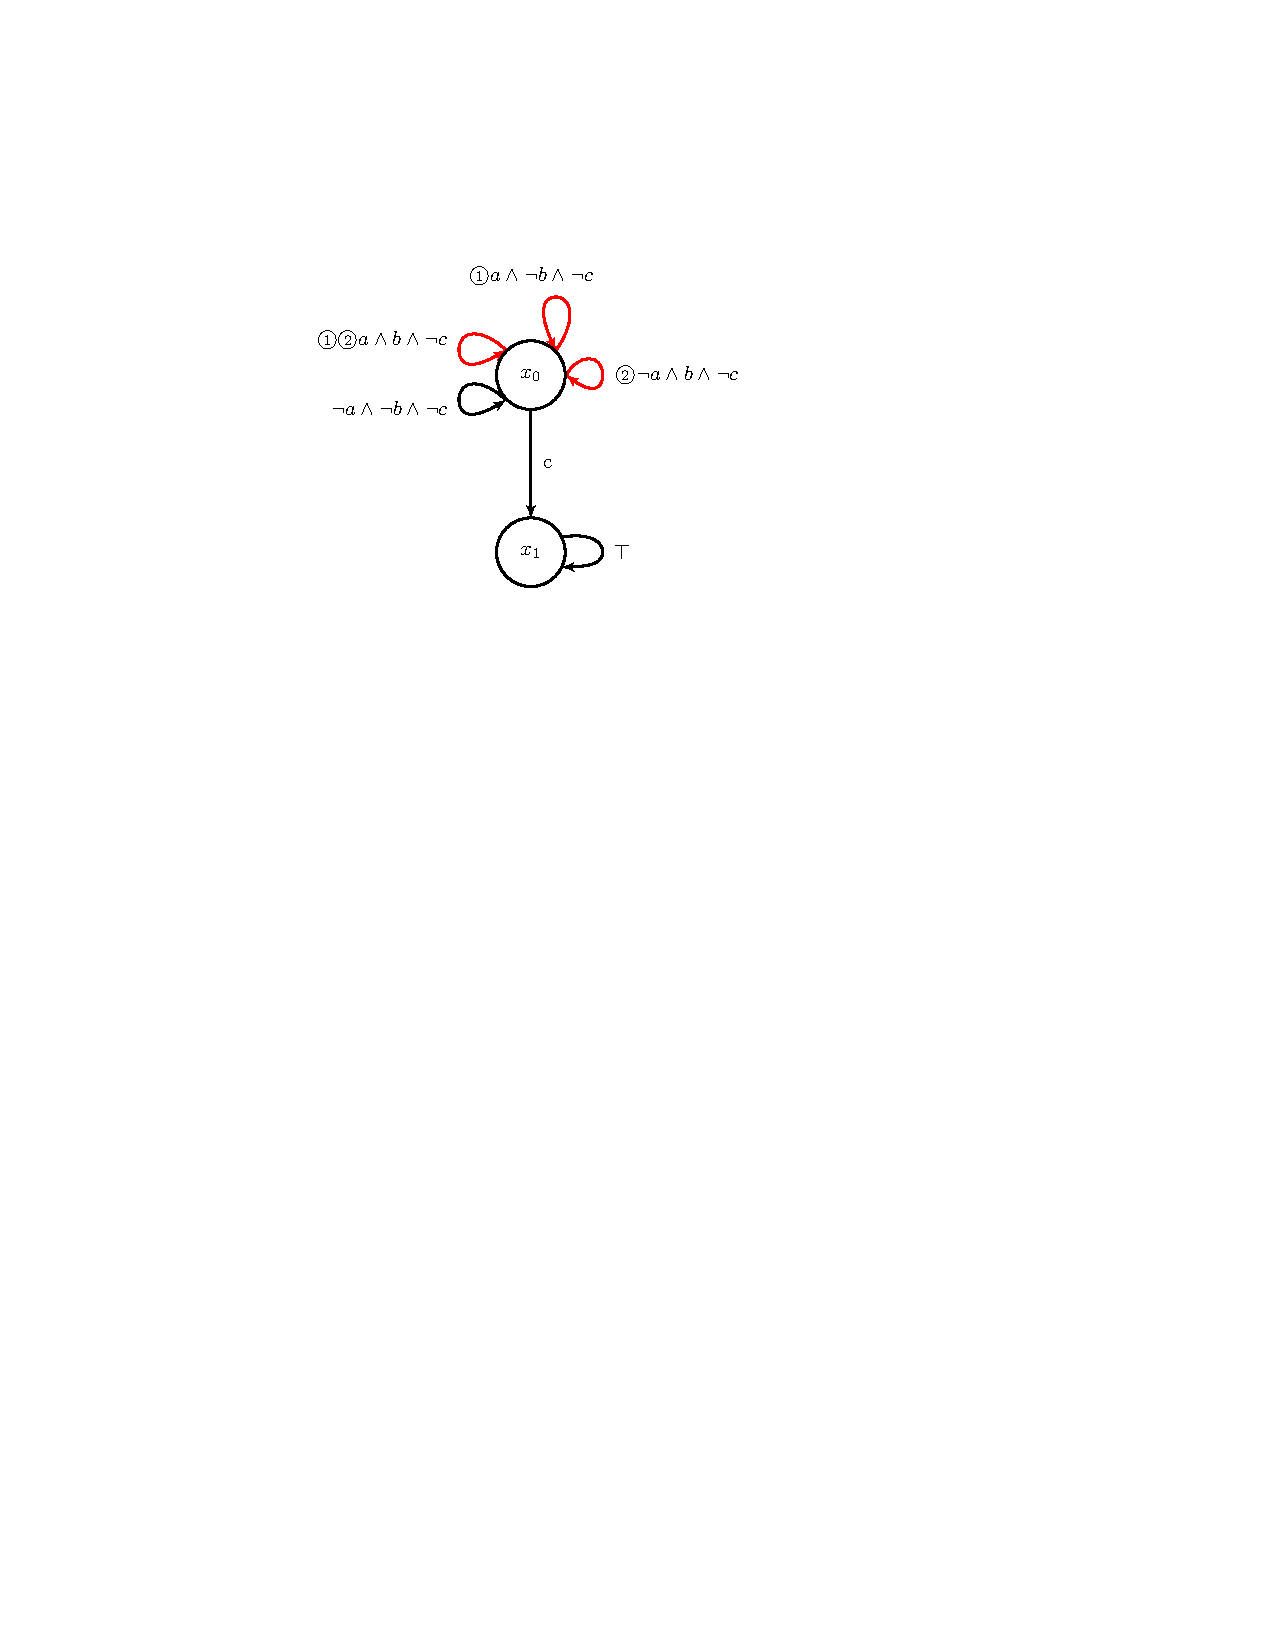
\includegraphics[bb=140 498 368 682,width=5cm]{automaton1.pdf}
   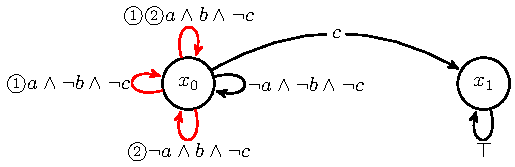
\includegraphics[bb=0 0 247 80,scale=0.65]{ldgba_original.pdf}
   \caption{The tLDGBA recognizing the LTL formula $\text{{\bf GF}}a \wedge \text{{\bf GF}}b \wedge \text{{\bf G}}\neg c$, where the initial state is $x_0$. Red arcs are accepting transitions that are numbered in accordance with the accepting sets they belong to.}
   % e.g., \textcircled{\scriptsize 1}$a \land \neg b \land \neg c$ means the transition labeled by it belongs to the accepting set $F_1$.}
   \label{automaton}
\end{figure}

\begin{figure}[htbp]
   \centering
%   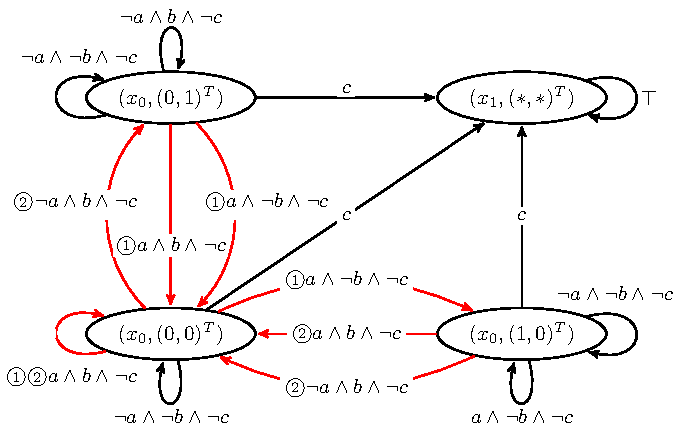
\includegraphics[bb=0 0 374 207,height=4cm, width=7cm]{ldgba.pdf}
   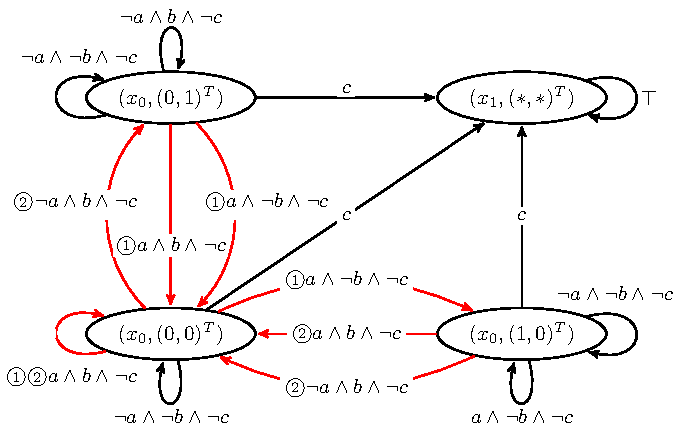
\includegraphics[bb=0 0 374 207,scale=0.6]{ldgba.pdf}
   \caption{The augmented automaton for the tLDGBA in Fig.~\ref{automaton} recognizing the LTL formula $\text{{\bf GF}}a \wedge \text{{\bf GF}}b \wedge \text{{\bf G}}\neg c$, where the initial state is $(x_0, (0,0)^T )$. Red arcs are accepting transitions that are numbered in accordance with the accepting sets they belong to. All states corresponding to $x_1$ are merged into $(x_1, (*,*)^T )$.}
   \label{automaton_aug}
\end{figure}
\end{comment}

In this section,
we apply the proposed method to a path planning problem of a robot in an environment consisting of eight rooms and one corridor as shown in Fig.\ \ref{Grid1}. The state $s_7$ is the initial state and the action space is specified with $\mathcal{A}(s) = \{ Right, Left, Up, Down \}$ for any state $s \neq s_4$ and $\mathcal{A}(s_4) = \{ to\_s_0, to\_s_1, to\_s_2, to\_s_3, to\_s_5, $ $to\_s_6, to\_s_7, to\_s_8 \}$, where $to\_s_i$ means attempting to go to the state $s_i$ for $i \in \{0,\ 1,\ 2,\ 3,\ 5,\ 6,\ 7,\ 8 \}$. The robot moves in the intended direction with probability 0.9 and it stays in the same state with probability 0.1 if it is in the state $s_4$. In the states other than $s_4$, it moves in the intended direction with probability 0.9 and it moves in the opposite direction with probability 0.1. If the robot tries to go to outside the environment, it stays in the same state. The labeling function is as follows.
\begin{align*}
      & L((s, act, s^{\prime})) =
      \left\{
      \begin{aligned}
        & \{ c \} &  & \text{if }s^{\prime} = s_i,\ i \in \{ 2,3,5,6 \}, \nonumber \\
        & \{ a \} &  & \text{if }(s,act,s^{\prime})=(s_4,to\_s_0,s_0), \nonumber \\
        & \{ b \} &  & \text{if }(s,act,s^{\prime})=(s_4,to\_s_8, s_8), \nonumber \\
        & \emptyset &  & \text{otherwise}.
      \end{aligned}
      \right.
    \end{align*}

In the example, the robot tries to take two transitions that we want to occur infinitely often, represented by arcs labeled by \{$a$\} and \{$b$\}, while avoiding unsafe transitions represented by the arcs labeled by \{{\it c}\}. This is formally specified by the LTL formula given by (\ref{ltl}).
The LTL formula requires the robot to keep on entering the two rooms $s_0$ and $s_8$ from the corridor $s_4$ regardless of the order of entries, while avoiding entering the four rooms $s_2$, $s_3$, $s_5$, and $s_6$.
% They have two accepting sets.
%We use Owl \cite{Owl} to obtain the tLDBA corresponding to the LTL formula.
The tLDGBA $B_{\varphi} = (X, x_{init},\Sigma,\delta,\mathcal{F})$ and its augmented automaton $\bar{B}_{\varphi} = (\bar{X},\bar{x}_{init},\bar{\Sigma},\bar{\delta},\bar{\mathcal{F}})$ are shown in Figs.\ \ref{automaton} and \ref{automaton_aug}, respectively.

Through the above scenario,
we compare our approach with 1) a case where we first convert the tLDGBA into a tLDBA, for which the augmentation makes no change, and thus a reward function in Definition \ref{def10} is based on a single accepting set; and
2) the method using a reward function based on the accepting frontier function \cite{HAK2019,HKAKPL2019}.
% In the method using tLDBA, the reward function is defined like Definition \ref{def10}, namely it is based on the one accepting set of the corresponding product MDP.
For the three methods, we use Q-learning\footnote{We employ Q-learning here but any algorithm that maximizes the discounted expected reward can be applied to our proposed method.} with $\varepsilon$-greedy policy and gradually reduce $\varepsilon$ to 0 to learn an optimal policy asymptotically.
We set the positive reward $r_p = 2$, the epsilon greedy parameter $ \varepsilon = \frac{0.95}{n_t(s^{\otimes})}$, where $n_t(s^{\otimes})$ is the number of visits to state $s^{\otimes}$ within $t$ time steps \cite{Singh1998}, and the discount factor $\gamma = 0.95$. The learning rate $\alpha$ varies in accordance with {\it the Robbins-Monro condition}. We train the agent in 10000 iterations and 1000 episodes for 20 learning sessions.

\begin{figure}[tbp]
 \centering
 \begin{tabular}{c}
  \begin{minipage}{0.5\hsize}
     \centering
%     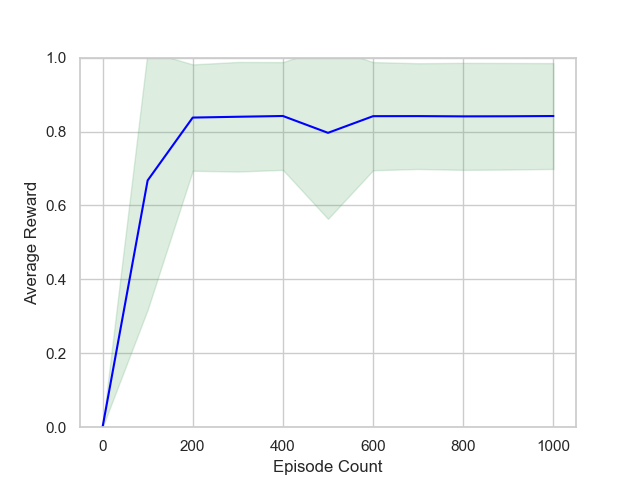
\includegraphics[width=4.5cm]{ep_1000_it_10000_MDP3_gamma_095_re2_ini22_nts_c095_20times.png}
     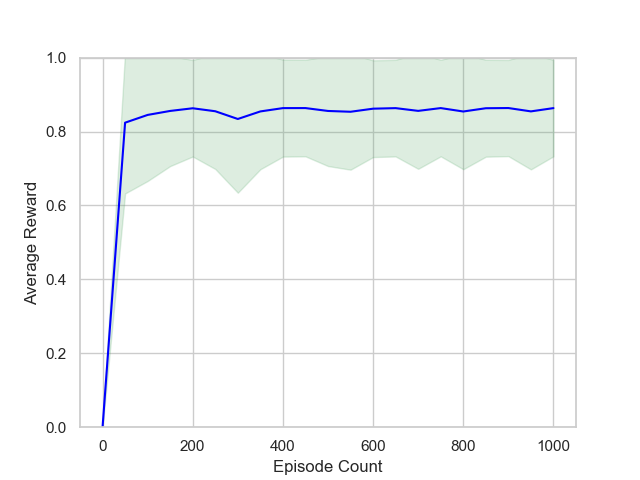
\includegraphics[bb=0 0 461 346, height = 3.8cm, width=5cm]{ep_1000_it_10000_MDP3_gamma_095_re2_ini22_nts_c095_100times_per50_no2.png}
 \end{minipage}

 \begin{minipage}{0.5\hsize}
   \centering
%   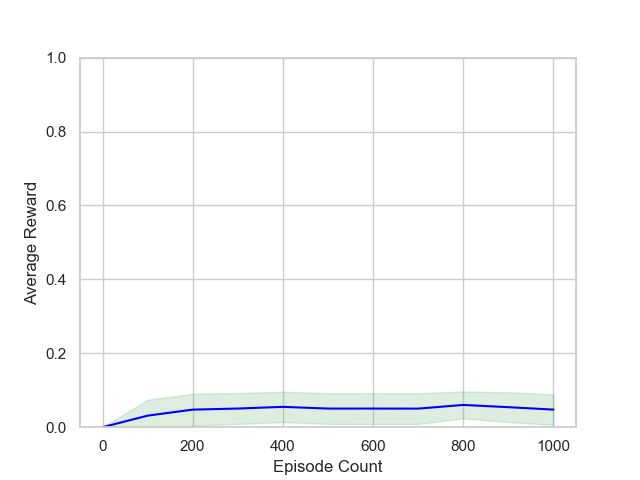
\includegraphics[width=4.5cm]{ep_1000_it_10000_MDP3_gamma_095_nts_c095_abate_20times.png}
   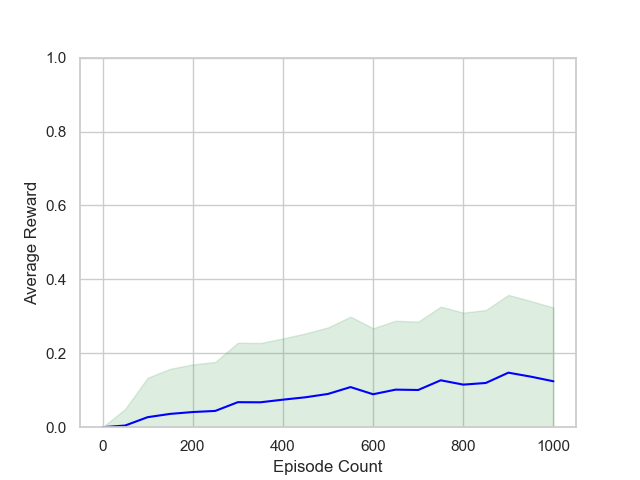
\includegraphics[bb=0 0 461 346, height = 3.8cm, width=5cm]{ep_1000_it_10000_MDP3_gamma_095_nts_c095_ldba_100times_per50.png}
 \end{minipage}
\end{tabular}
 \caption{The mean of average reward in each episode for 20 learning sessions obtained from our proposed method (left) and the method using tLDBA (right). They are plotted per 50 episodes and the green areas represent the range of standard deviations. }
 \label{result}
\end{figure}

\begin{figure}[tbp]
	\centering
	\begin{tabular}{c}

		\begin{minipage}{0.499\hsize}
		\centering
			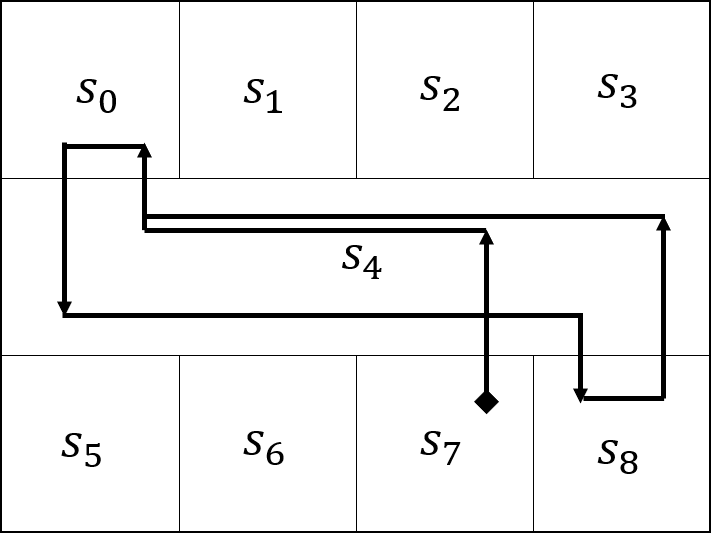
\includegraphics[bb=0 0 341 256, height = 2.7cm,
			width=3.5cm]{proposed_policy.png}
		\end{minipage}

		\begin{minipage}{0.499\hsize}
			\centering
			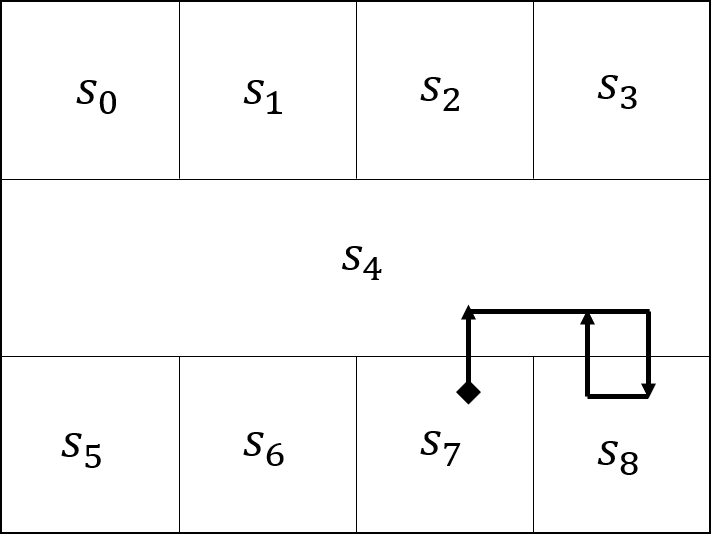
\includegraphics[bb=0 0 341 257, height = 2.7cm,
			width=3.5cm]{Abate_policy.png}
		\end{minipage}
	\end{tabular}

	\caption{The optimal policy obtained from our proposed method (left) and the method in \cite{HAK2019, HKAKPL2019} (right).}
	\label{optimal}
\end{figure}

%We conduct the same example with their method using the tLDGBA instead.
\subsection*{Results}
\textit{1) }
Fig.\ \ref{result} shows the average rewards obtained by our proposed method and the case using a tLDBA $B^{\prime}_{\varphi}$ converted from $\varphi$, respectively.
%Note that the theoretical convergence values of the average reward for both methods are different.
Both methods eventually acquire an optimal policy satisfying $\varphi$. As shown in Fig.\ \ref{result}, however, our proposed method converges faster. This is because the order of entrance to the rooms $s_0$ and $s_8$ is determined according to the tLDBA.
%This is because the ratio of the number of accepting transitions to that of all transitions in $\bar{B}_{\varphi}$ is greater than $B^{\prime}_{\varphi}$.
Moreover, the number of transitions with a positive reward in $\bar{B}_\varphi$ is larger than that in $B_\varphi'$.

% \subsubsection{vs. tLDGBA with accepting frontier function}
%  In, the accepting frontier function is proposed.
\textit{2) }
 We use the accepting frontier function \cite{HAK2019,HKAKPL2019} for the tLDGBA $Acc : \delta \times 2^{\delta} \rightarrow 2^{\delta} $. Initializing a set of transitions $ \mathbb{F} $ with the set of the all accepting transitions in $B_{\varphi}$, the function receives the transition $(x, \sigma, x^{\prime})$ that occurs and the set $\mathbb{F}$. If $(x, \sigma, x^{\prime})$ is in $\mathbb{F}$, then $Acc$ removes the accepting sets containing $(x, \sigma, x^{\prime})$ from $\mathbb{F}$. For the product MDP of the MDP $M$ and the tLDGBA $B_{\varphi}$, the reward function is based on the removed sets of $B_{\varphi}$.

Fig.\ \ref{optimal} shows the optimal policies obtained by our proposed method and the method in \cite{HAK2019,HKAKPL2019}\footnote{We obtain the same result even with a state-based LDGBA.}, respectively.
The policy obtained by the method with the accepting frontier function fails to satisfy the LTL specification
% The result for the method in \cite{HAK2019,HKAKPL2019} is
because it is impossible with $B_{\varphi}$ shown in Fig.\ \ref{automaton} that the transitions labeled with $\{ a \}$ and $\{ b \}$ occur from $s_4$ infinitely often by any positional policy. More specifically, the state of $B_{\varphi}$ is always $x_0$ while the agent does not move to bad states $s_2$, $s_3$, $s_5$, and $s_6$.
Whenever the agent is in $s_4$, therefore, the product MDP is always in $(s_4, x_0)$ unless one of the bad states are visited.
% while the agent is in $s_4$.
Thus, the agent cannot visit both of $s_0$ and $s_8$ by a deterministic action selection at $s_4$.
On the other hand, our proposed method can recognize the previous visits.
Thus, our proposed method can synthesize a positional policy satisfying $\varphi$ on the product MDP, while the method in \cite{HAK2019, HKAKPL2019} cannot. In order to obtain a positional policy satisfying the LTL formula $\varphi$ with the method in \cite{HAK2019,HKAKPL2019} in this example, we have to refine the tLDGBA shown in Fig.~\ref{automaton} heuristically, e.g., by adding states with which the order of occurrences of accepting transitions is recognized.
%However, such heuristic redundancy may make rewards sparser and a search space larger than necessary.
% Therefore, the method in \cite{HAK2019} may not synthesize positional policies satisfying LTL specifications on the product MDP depending on the settings of MDPs or LTL specifications.


%%%%%%%%%%%% 4th Chapter %%%%%%%%%%%%%%%%%%%%%%%%%%%%%%%%%%%%%%%%%%%%%%%%%%%
\chapter{Reinforcement learning based supervisor synthesis for LTL specifications}


\begin{definition}
  Given an augmented tLDBA $\bar{B}_{\varphi} = (\bar{X}, \bar{x}_{init},\bar{\Sigma},\bar{\delta},\bar{\mathcal{F}})$ and a DES $D$, a tuple $D \otimes \bar{B}_{\varphi} = D^{\otimes} = (S^{\otimes}, E^{\otimes}, s_{init}^{\otimes}, P^{\otimes}_T, P^{\otimes}_E, \delta^{\otimes}, {\mathcal F}^{\otimes})$ is a product DES, where
  $S^{\otimes} = S \times \bar{X}$ is the finite set of states and we represent $s$ and $\bar{x}$ corresponding with $s^{\otimes} = (s,\bar{x}) \in S^{\otimes}$ as $\mysps$ and $\myspq$, respectively; $E^{\otimes}=E \cup \{ \varepsilon_{\bar{x}^{\prime}} ; \exists \bar{x}^{\prime} \text{s.t.} (\bar{x}, \varepsilon, \bar{x}^{\prime}) \in \bar{\delta} \} $ is the finite set of events, where $\varepsilon_{\bar{x}^{\prime}}$ is the event that represents an $\varepsilon$-transition to $\bar{x}^{\prime} \in \bar{X}$; $s_{init}^{\otimes} = (s_{init},\bar{x}_{init})$ is the initial states, $P^{\otimes}_T : S^{\otimes} \times S^{\otimes} \times E^{\otimes} \rightarrow [0,1]$ is the transition probability defined as
  \begin{align}
    P^{\otimes}_T(s^{\otimes \prime} | s^{\otimes}, e) =
    \left\{
    \begin{aligned}
      &P_T(s^{\prime} | s, e) &   &\text{if}\  (\bar{x}, L((s,e,s^{\prime})), \bar{x}^{\prime}) \in \bar{\delta}, e \in \mathcal{E}(s) \\
      &1 &   &\text{if}\ s=s^{\prime}, (\bar{x}, \varepsilon, \bar{x}^{\prime}) \in \delta, e= \varepsilon_{\bar{x}^{\prime}} \\
      &0 &   &\text{otherwise} ,
    \end{aligned}
    \right. \nonumber
  \end{align}
  where $s^{\otimes} = (s,(x,v))$ and $s^{\otimes \prime} = (s^{\prime}, (x^{\prime}, v^{\prime}))$.
  $P^{\otimes}_E : E^{\otimes} \times S^{\otimes} \times 2^{E^{\otimes}} \rightarrow [0,1]$ is the probability of the occurrence of the event defined as $P^{\otimes}_E(e | s^{\otimes}, \pi) = P_E(e | s, \pi)$, $\delta^{\otimes} = \{ (s^{\otimes}, e, s^{\otimes \prime}) \in S^{\otimes} \times E^{\otimes} \times S^{\otimes} ; P^{\otimes}_T(s^{\otimes \prime} | s^{\otimes}, e) > 0 \}$ is the set of transitions, and ${\mathcal F}^{\otimes} = \{ \bar{F}^{\otimes}_1, \ldots ,\bar{F}^{\otimes}_n \}$ is the acceptance condition, where $\bar{F}^{\otimes}_i = \{ ((s,\bar{x}), e, (s^{\prime}, \bar{x}^{\prime})) \in \delta^{\otimes}\ ;\ (\bar{x}, L(s,e,s^{\prime}), \bar{x}^{\prime}) \in \bar{F}_i \}$ for each $ i \in \{ 1, \ldots ,n \}$.
\end{definition}

\begin{definition}
  The two reward functions $\mathcal{R}_1 : S^{\otimes} \times 2^{E^{\otimes}} \rightarrow \mathbb{R}$ and $\mathcal{R}_2 : S^{\otimes} \times E^{\otimes} \times S^{\otimes} \rightarrow \mathbb{R}$ are defined as follows.
  \begin{align}
    \mathcal{R}_1 (s^{\otimes}, \pi) =
    \left\{
    \begin{aligned}
      & r_{n}|\pi| & &\text{if} \ \myspq \notin SinkSet , \\
      & 0 & &\text{otherwise},
    \end{aligned}
    \right.
  \end{align}
  where $|E|$ means the number of elements in the set $E$ and $r_{n}$ is a positive value.
  \begin{align}
    \mathcal{R}_2(s^{\otimes}, e, s^{\otimes \prime}) =
    \left\{
    \begin{aligned}
      &r_p & & \text{if}\ \exists j \in \! \{ 1, \ldots ,n \},\ (s^{\otimes}, e, s^{\otimes \prime}) \in \bar{F}^{\otimes}_j \!,\\
      &r_{sink} & & \text{if}\ \myspdq \in SinkSet,\\
      &0 & & \text{otherwise},
    \end{aligned}
    \right.
  \end{align}
  where $r_p$ and $r_{sink}$ are the positive and negative value, respectively.
  \label{reward_def}
\end{definition}

\section{Learning Algorithm}
We make the supervisor learn how to give the control patterns to satisfy an LTL specification while keeping costs associated with disabled events low. We use Q-learning to estimate the function $T^{\ast}$. We then use Bayesian inference to robustly estimate the probability $P_E$. For the inference, we model $P_E$ as Categorical distribution as $p^k_{s,\pi,e}$, where $p^k_{s,\pi,e}$ represents the estimated probability of $P_E(e|s,\pi)$ at the time step $k$ and the prior distribution $\phi^k_{s,\pi}$ for the distribution of the parameter of $p^k_{s,\pi,e}$ is defined as Dirichlet.
%Let $\mathcal{P}_{s,\pi}$ be the collection of the estimated probabilities of $P_E(e|s,\pi)$ with respect to all $e \in \pi$.

In the following, we distinguish events by numbering them as $\{ e^1, \ldots, e^{|E|} \}$ . In order to reflect the events disabled by the supervisor on the estimated probability of an event occurrence, we introduce the function $RestProb : (0,1)^{|E|} \times 2^E \rightarrow [0,1]^{|E|}$ defined as

\begin{align}
  RestProb(\phi^k_{s,\pi},\pi)_i =
  \left\{
  \begin{aligned}
    & \frac{\phi^{k,i}_{s,\pi}}{\sum_{e^j \in \pi} \phi^j_{s,\pi}} \  &\text{if}\ e^i \in \pi,\\
    &0   \ &\text{otherwise},
  \end{aligned}
  \right.
\end{align}
where $\phi^{k,i}_{s,\pi}$ is the $i$-th element of $\phi^k_{s,\pi}$ and $RestProb(\phi^k_{s,\pi},\pi)_i$ is the $i$-th element of $RestProb(\phi^k_{s,\pi},\pi)$.

We denote the probability vector of an event occurrence at the time step $k$ as $p^k_{s,\pi} = (p^k_{s,\pi,e^1}, \ldots, p^k_{s,\pi,e^{|E|}})$, where $s \in S$ and $\pi \in \mathcal{E}(s)$ is the state and the control pattern at the time step $k$. Let $n^k_{s,\pi,e}$ be the number of the occurrence of the event $e \in E$ up to the time step $k$ at the state $s \in S$ under the control pattern $\pi \in \mathcal{E}(s)$ and let $n^k_{s,\pi} = (n^k_{s,\pi,e_1}, \ldots, n^k_{s,\pi,e_{|E|}})$.
% and let $\bar{p}^k_{s,\pi}$ denote the expected value of $p^k_{s,\pi}$.
We sample the parameter $\phi^k_{s,\pi}$ of the posterior distribution of an event occurrence from the Dirichlet distribution $Dir(\cdot|n^k_{s,\pi})$. Then, we obtain the estimated probability vector $p^k_{s,\pi}$ of an event occurrence by $RestProb$ from the sampled parameter $\phi^k_{s,\pi}$ and the control pattern $\pi$.
%We repeat the procedure until $||p^k_{s,\pi} - \bar{p}^k_{s,\pi}||_1 < \xi^k_{s,\pi}$ holds.

The overall procedure of the inference is shown in Algorithm \ref{bayes}.

\begin{algorithm}[H]
 \caption{$P_E$ inference.}
 \begin{algorithmic}[1]
 \renewcommand{\algorithmicrequire}{\textbf{Input:}}
 \renewcommand{\algorithmicensure}{\textbf{Output:}}
 \REQUIRE the event occurrence count $n^k_{s,\pi}$, a threshold $\xi^k_{s,\pi}$ for $p^k_{s,\pi}$
 \ENSURE  the posterior distribution $p^k_{s,\pi}$
  %\REPEAT
  \STATE $\phi^k_{s,\pi} \sim Dir(\cdot|n^k_{s,\pi})$
  \STATE $p^k_{s,\pi} = RestProb(\phi^k_{s,\pi},\pi)$
  %\UNTIL $||p^k_{s,\pi} - \bar{p}^k_{s,\pi}||_1 < \xi^k_{s,\pi}$
 \end{algorithmic}
 \label{bayes}
 \end{algorithm}

Under the estimation of $P_E$, we use TD-learning to estimate $Q^{\ast}$ with the TD-error defined as $\mathcal{R}_1(s^{\otimes},\pi) + \sum_{e \in \pi} p_{\mysps,\pi,e} T(s^{\otimes},e) - Q(s^{\otimes},\pi)$.

We show the overall procedure of the learning algorithm in Algorithm \ref{alg1}.

\begin{algorithm}[H]
 \caption{RL-based synthesis of a supervisor satisfying the given LTL specification.}
 \begin{algorithmic}[1]
 \renewcommand{\algorithmicrequire}{\textbf{Input:}}
 \renewcommand{\algorithmicensure}{\textbf{Output:}}
 \REQUIRE LTL formula $\varphi$, DES $M$
 \ENSURE  optimal supervisor $SV^{\ast}$ on the product DES $M^{\otimes}$
  \STATE Convert $\varphi$ into tLDGBA $B_{\varphi}$.
  \STATE Augment $B_{\varphi}$ to $\bar{B}_{\varphi}$.
  \STATE Construct the product DES $M^{\otimes}$ of $M$ and $\bar{B}_{\varphi}$.
  \STATE Initialize $T:S^{\otimes} \times E^{\otimes} \rightarrow \mathbb{R}$.
  \STATE Initialize $Q:S^{\otimes} \times 2^{E^{\otimes}} \rightarrow \mathbb{R}$.
  \STATE Initialize $n:S \times 2^{E} \times E \rightarrow \mathbb{R}$.
  \STATE initialize $\xi:S \times 2^{E} \rightarrow \mathbb{R}$.
  \STATE Initialize episode length $L$.
  \WHILE {$Q$ is not converged}
  \STATE $s^{\otimes} \leftarrow (s_{init},(x_{init},\bm{0}))$.
  \STATE $t \leftarrow 0$
  \WHILE {$t <L$ and $\myspq \notin SinkSet$ }
  \STATE Choose the control pattern $\pi \in 2^{\mathcal{E}(s^{\otimes})}$ by the supervisor $SV$.
  \STATE Observe the occurrence of the event $e \in E$.
  \STATE Observe the next state $s^{\otimes \prime}$.
  \STATE $T(s^{\otimes},e) \leftarrow (1-\alpha)T(s^{\otimes},e) + \alpha \{\mathcal{R}_2(s^{\otimes},e,s^{\otimes \prime}) + \gamma \max_{\pi^{\prime} \in 2^{\mathcal{E}(s^{\otimes \prime})}}Q(s^{\otimes \prime},\pi^{\prime})\}$
  \STATE $n(\mysps, \pi, e) \leftarrow n(\mysps, \pi, e) + 1$
  \STATE Obtain $p_{\mysps,\pi}$ from $n$ by the $P_E$ inference.
  \STATE $Q(s^{\otimes},\pi) = (1-\beta)Q(s^{\otimes},\pi) + \beta \{\mathcal{R}_1(s^{\otimes},\pi) + \sum_{e \in \pi} p_{\mysps,\pi,e} T(s^{\otimes},e)$\}
  \STATE $s^{\otimes} \leftarrow s^{\otimes \prime}$
  \STATE $t \leftarrow t + 1$
  %\STATE Update $\xi(s^{\otimes}, \pi)$
  \ENDWHILE
  \ENDWHILE
 \end{algorithmic}
 \label{alg1}
 \end{algorithm}

\section{Example}
We evaluate the algorithm by the maze of the cat and the mouse shown in Fig.\ \ref{cat_mouse}. At the beginning, we define the settings for the example. The corresponding DES is as follows. The state set is $S = \{ (s^{cat}, s^{mouse}) ; s^{cat},s^{mouse} \in \{ s_0,s_1,s_2,s_3 \} \}$. The set of events (to open the corresponding door) is $E = \{ m_0, m_1, m_2, m_3, c_0, c_1, c_2, c_3 \}$, where $E_{c} = \{ m_0, m_1, m_2, m_3, c_0, c_1, c_2 \}$ and $E_{uc} = \{ c_3 \}$ and $\mathcal{E}(s) = E$ for any $s \in S$. The initial state is $s_{init} = (s_0, s_2)$. If the door of the room with the cat (resp., mouse) opens, the cat (resp., mouse) moves, with probability 0.95, to the room next to the room through the door or stays in the same room with probability 0.05. Otherwise, the cat (resp., mouse) stays in the same room with probability 1. The labeling function is

\begin{align}
   L((s, a, s^{\prime})) =
    \left\{
    \begin{aligned}
      & \{ a \} &  & \text{if }s_c^{\prime} = s_1, \nonumber \\
      & \{ b \} &  & \text{if }s_m^{\prime} = s_1, \nonumber \\
      & \{ c \} &  & \text{if }s_c^{\prime} = s_m^{\prime}, \nonumber \\
      & \emptyset &  & \text{otherwise},
    \end{aligned}
    \right.
\end{align}
where $s_c^{\prime}$ and $s_m^{\prime}$ is the next room where the cat and the mouse is, respectively, i.e., $s^{\prime} = (s_c^{\prime},s_m^{\prime})$.

In the example, we want the supervisor to learn to give control patterns satisfying that the cat and the mouse take the food in the room 1 ($s_1$) avoiding they come across. This is formally specified by the following LTL formula.
\begin{align*}
  \varphi = \text{{\bf GF}}a \wedge \text{{\bf GF}}b \wedge \text{{\bf G}}\neg c.
\end{align*}
The tLDGBA $B_{\varphi} = (X, x_{init},\Sigma,\delta,\mathcal{F})$ corresponding to $\varphi$ is shown in Fig.\ \ref{tldba}. $B_{\varphi}$ has the acceptance condition of two accepting sets.

We use $\varepsilon$-greedy policy and gradually reduce $\varepsilon$ to 0 to learn an optimal supervisor asymptotically.
We set the rewards $r_p = 10$, $r_{n} = 0.1, 0.7, and 1.2$, and $r_{sink} = -1000$; the epsilon greedy parameter $ \varepsilon = \frac{1}{ \sqrt{episode} }$, where $episode$ is the number of the current episode; and the discount factor $\gamma = 0.99$. %$\xi^k_{s^{\otimes},\pi}$ is initially set to 1 and changes to 0.6 during 1/3 to 2/3 of all episodes and to 0.3 after 2/3 of all episodes for any $(s^{\otimes},\pi) \in S^{\otimes} \times 2^{E^{\otimes}}$.
The learning rate $\alpha$ and $\beta$ vary in accordance with {\it the Robbins-Monro condition}. We train supervisors 5000 iterations and 15000 episodes.

Fig.\ \ref{result1} shows the estimated optimal state values at the initial state $V(s^{\otimes}_{init})$ with $r_{n} = 0.1, 0.7,$ and $1.2$, respectively, for each episode when learning 5000 iterations and 15000 episodes by the algorithm \ref{alg1}.
Fig.\ \ref{sim1} shows the average rewards from $\mathcal{R}_2$ and the average rewards from $\mathcal{R}_1$ with $r_{n} = 0.1, 0.7,$ and $1.2$, respectively, of 5000 iterations and 1000 episodes by the supervisor obtained from the learning.

Fig.\ \ref{result1} suggests the three supervisors becomes optimal as the episode progresses.
Fig.\ \ref{sim1} suggests the three supervisors obtained from the learning satisfy $\varphi$ and there is no sink recurrent class under the supervisors. The latter is implied by the stable average rewards.
Furthermore, Fig.\ \ref{sim1} suggests that there is a trade-off between the frequency of visits to accepting sets of a augmented tLDGBA corresponding to a given LTL formula and the number of enabling events. Moreover, we can consider how much we see it important to enable events and how often the event occurs that leads to the satisfaction of a given LTL formula by changing the magnitude of the reward for control patterns and the reward for the LTL formula relatively.

\begin{figure}[htbp]
   \centering
   \vspace{2mm}
%   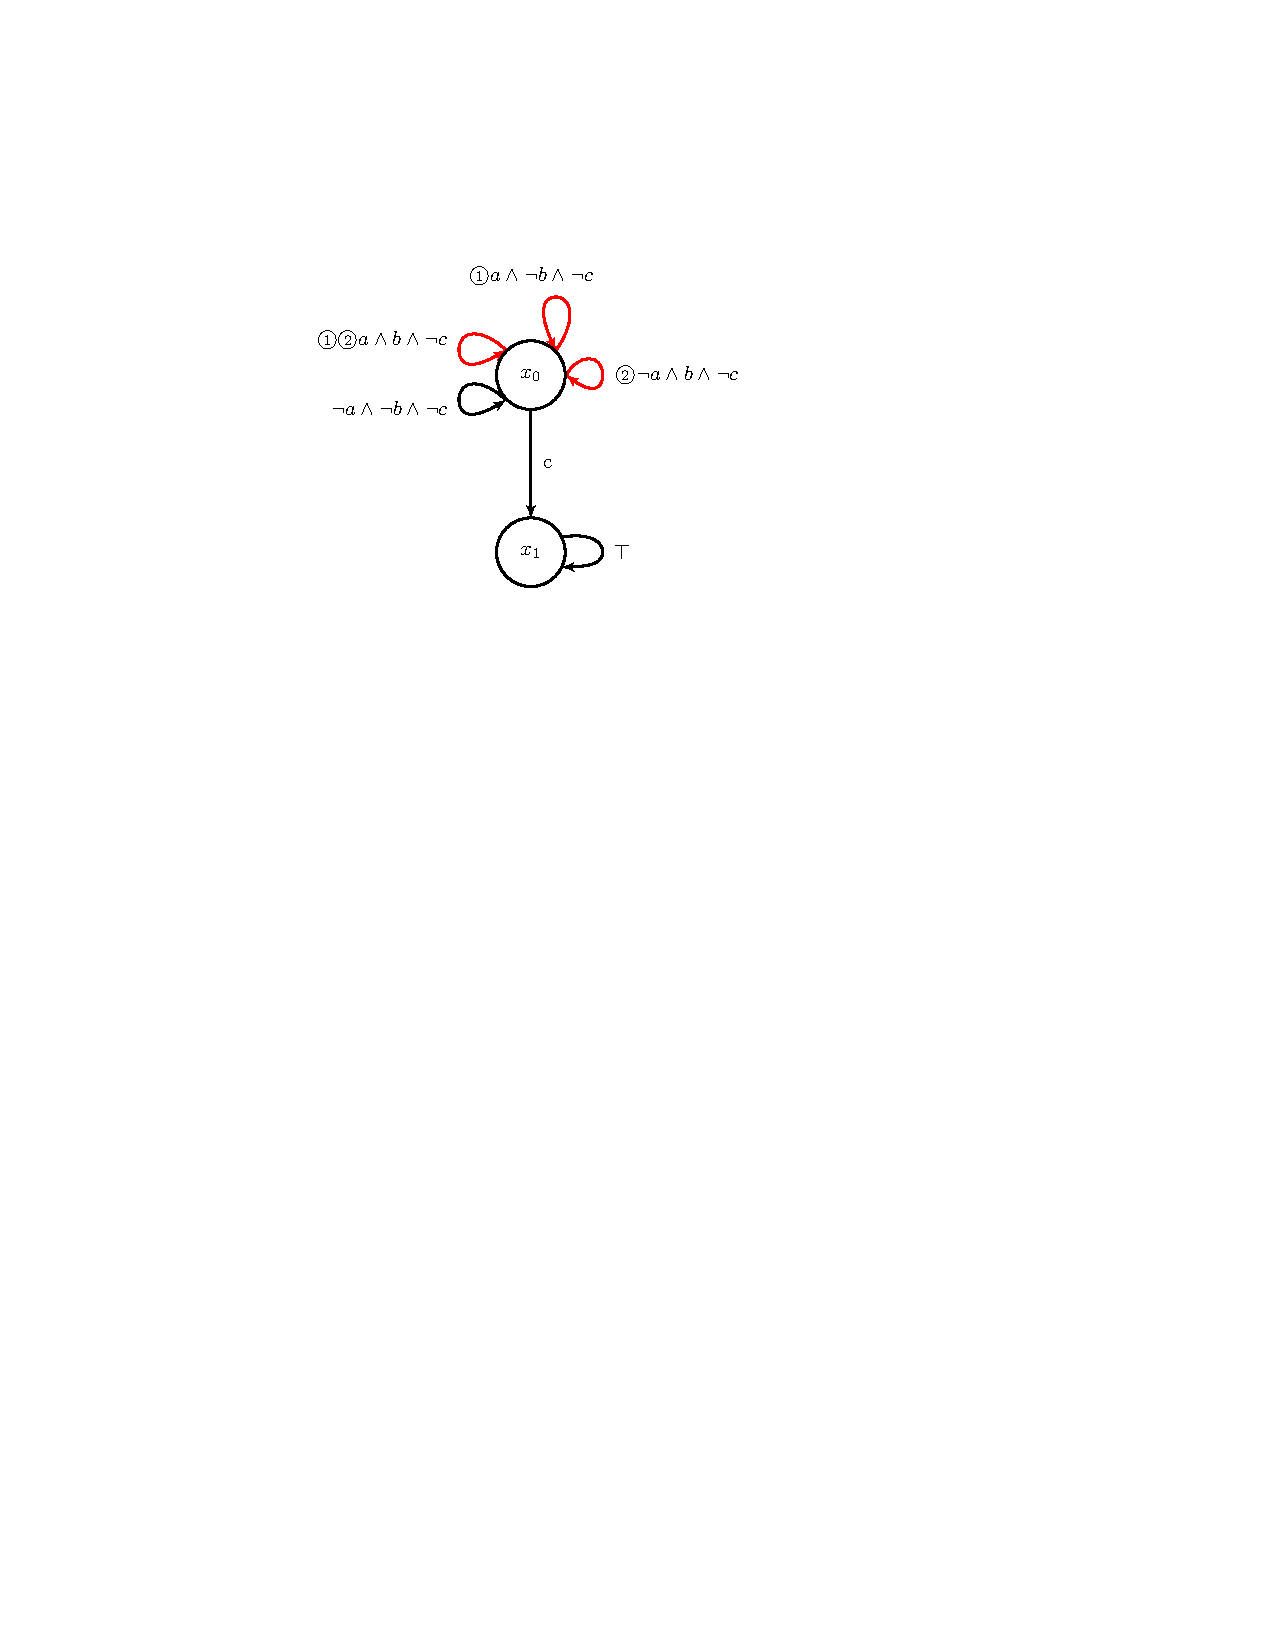
\includegraphics[bb=140 498 368 682,width=5cm]{automaton1.pdf}
   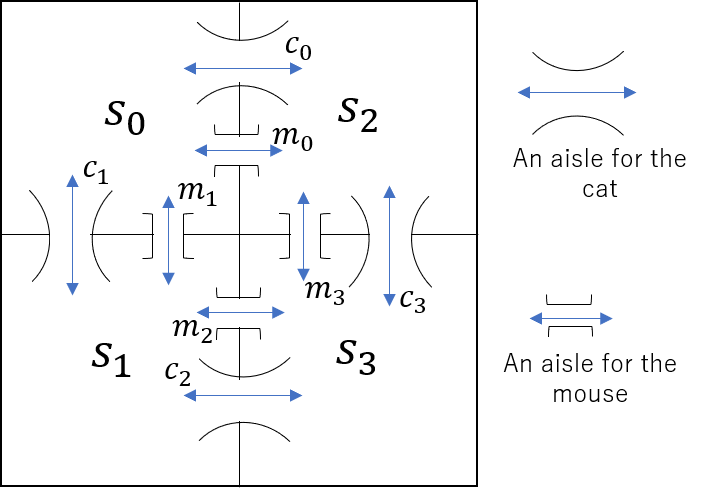
\includegraphics[width=7cm]{cat_mouse.png}
   \caption{The maze of the cat and the mouse. the initial state of the cat and the mouse is $s_0$ and $s_2$, respectively. the food for them is in the room 1 ($s_1$).}
   \label{cat_mouse}
\end{figure}

\begin{figure}[htbp]
   \centering
   \vspace{2mm}
%   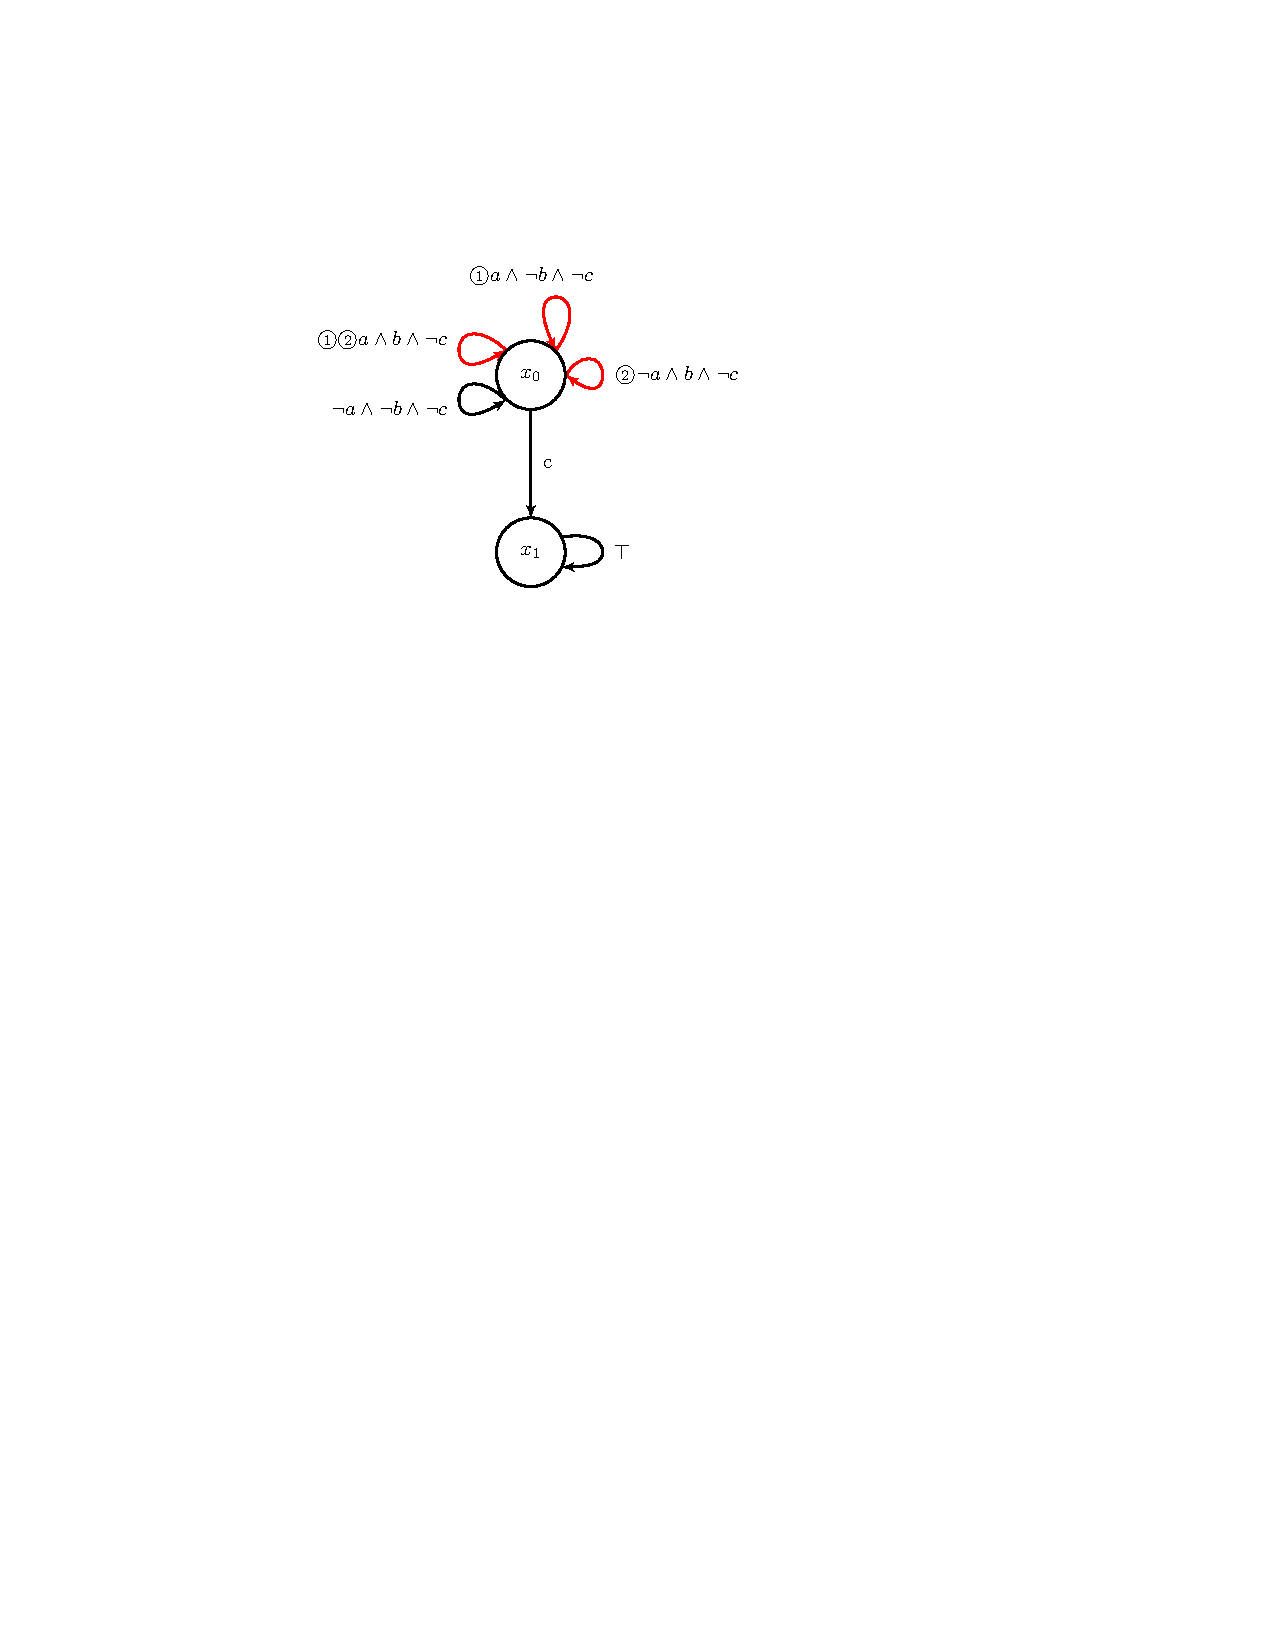
\includegraphics[bb=140 498 368 682,width=5cm]{automaton1.pdf}
   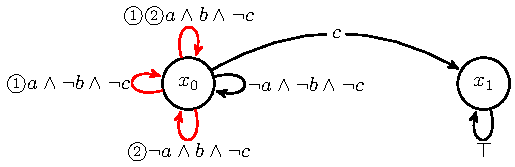
\includegraphics[bb=0 0 247 80,scale=0.85]{ldgba_original.pdf}
   \caption{The tLDGBA recognizing the LTL formula $\text{{\bf GF}}a \wedge \text{{\bf GF}}b \wedge \text{{\bf G}}\neg c$, where the initial state is $x_0$. Red arcs are accepting transitions that are numbered in accordance with the accepting sets they belong to, e.g., \textcircled{\scriptsize 1}$a \land \neg b \land \neg c$ means the transition labeled by it belongs to the accepting set $F_1$.}
   \label{tldba}
\end{figure}

\begin{figure}[H]
   \centering
   \vspace{2mm}
%   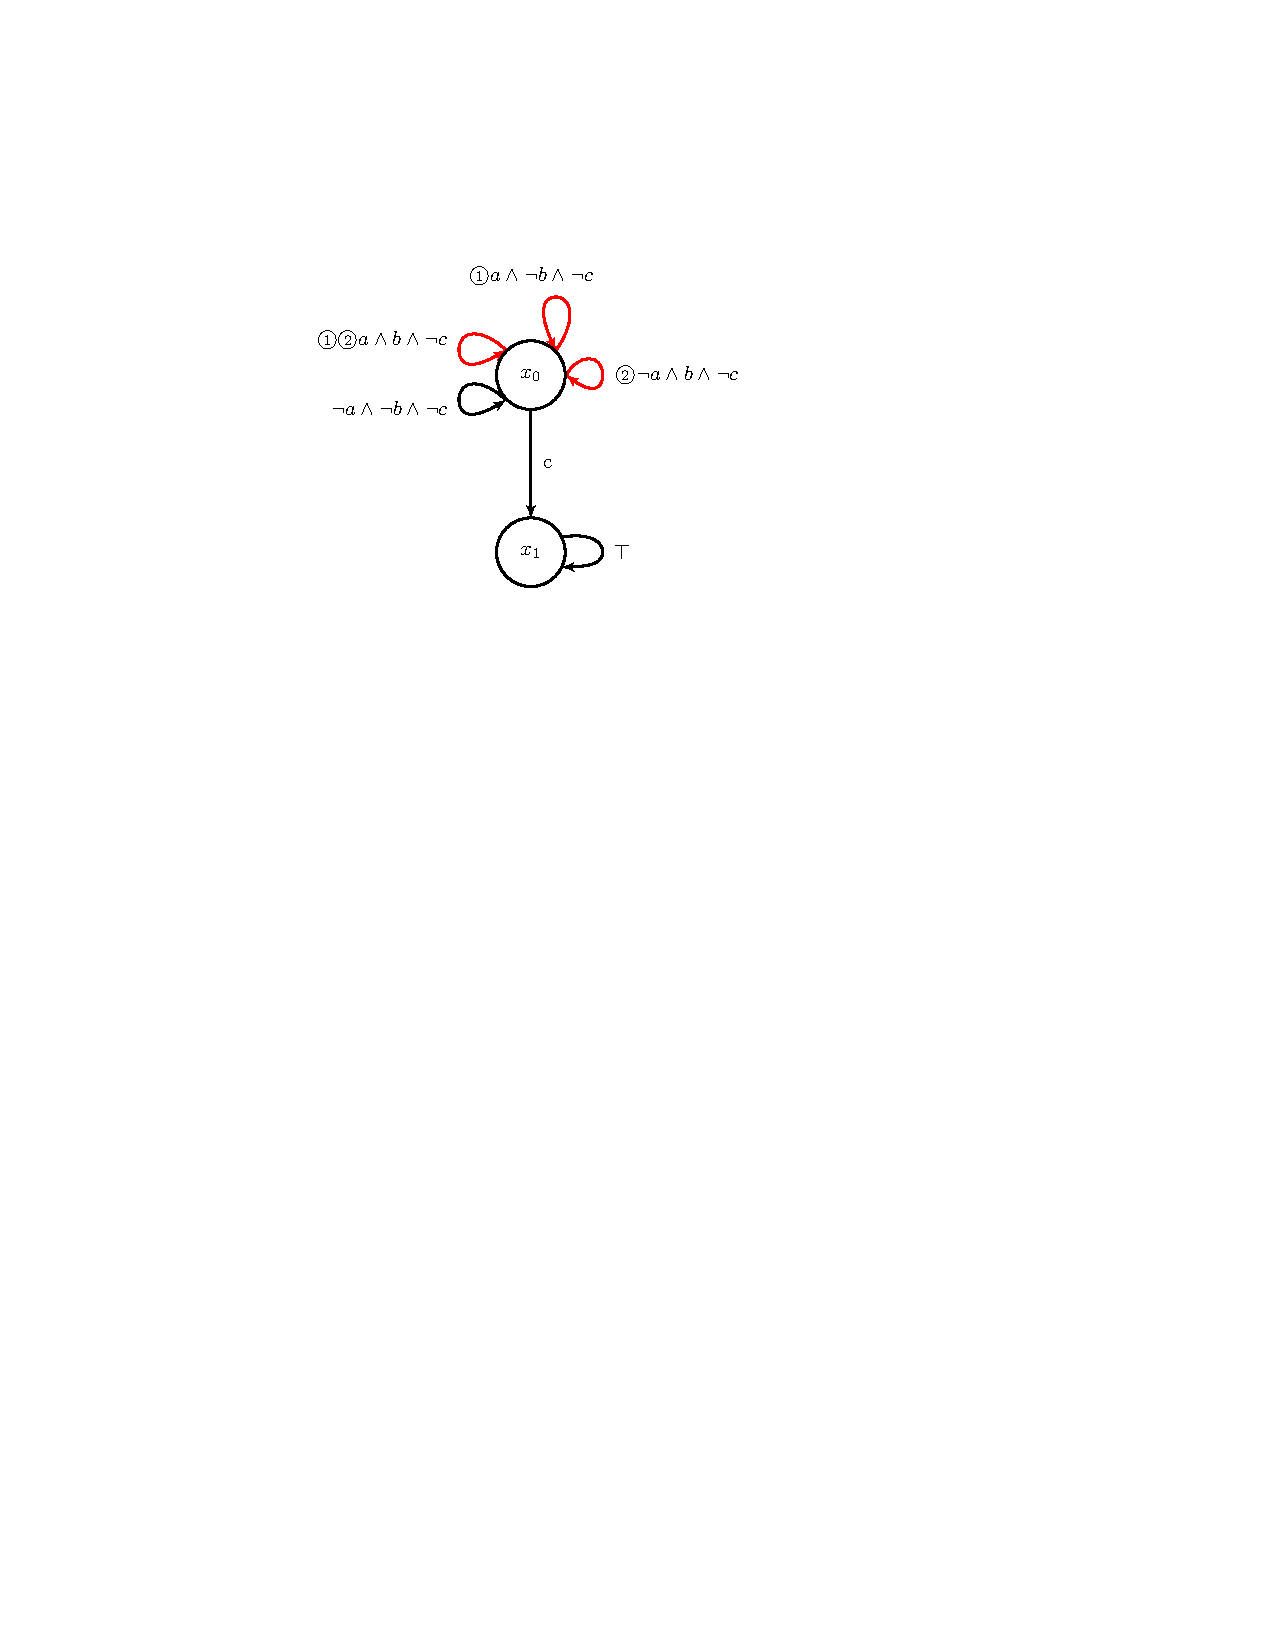
\includegraphics[bb=140 498 368 682,width=5cm]{automaton1.pdf}
   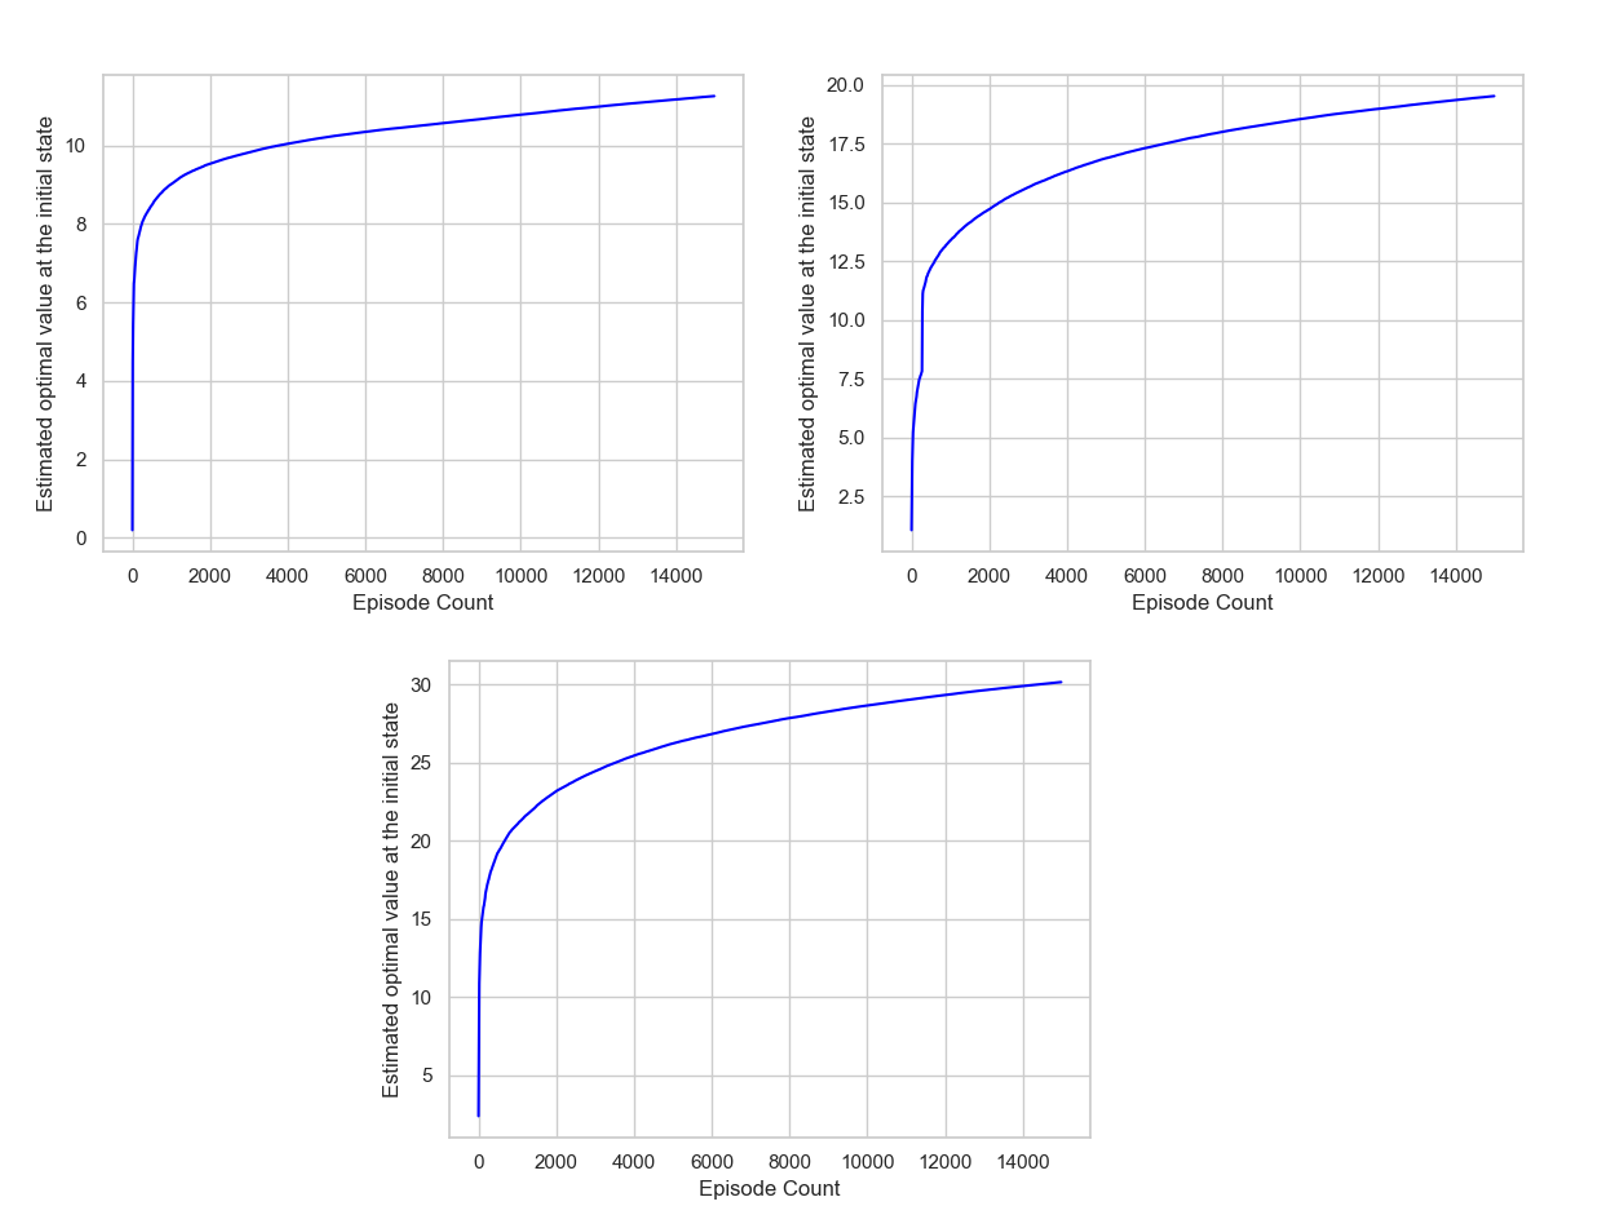
\includegraphics[width = 12cm]{max_Q_value_15000_5000_rn_all_rsink_1000.png}
   \caption{The estimated optimal state values at the initial state $V(s^{\otimes}_{init})$ with $r_{n} = 0.1$ (left above), $r_n = 0.7$ (right above), and $r_n = 1.2$ (below) when using Algorithm \ref{alg1}.}
   \label{result1}
\end{figure}

\begin{figure}[H] %htbp
   \centering
   \vspace{2mm}
%   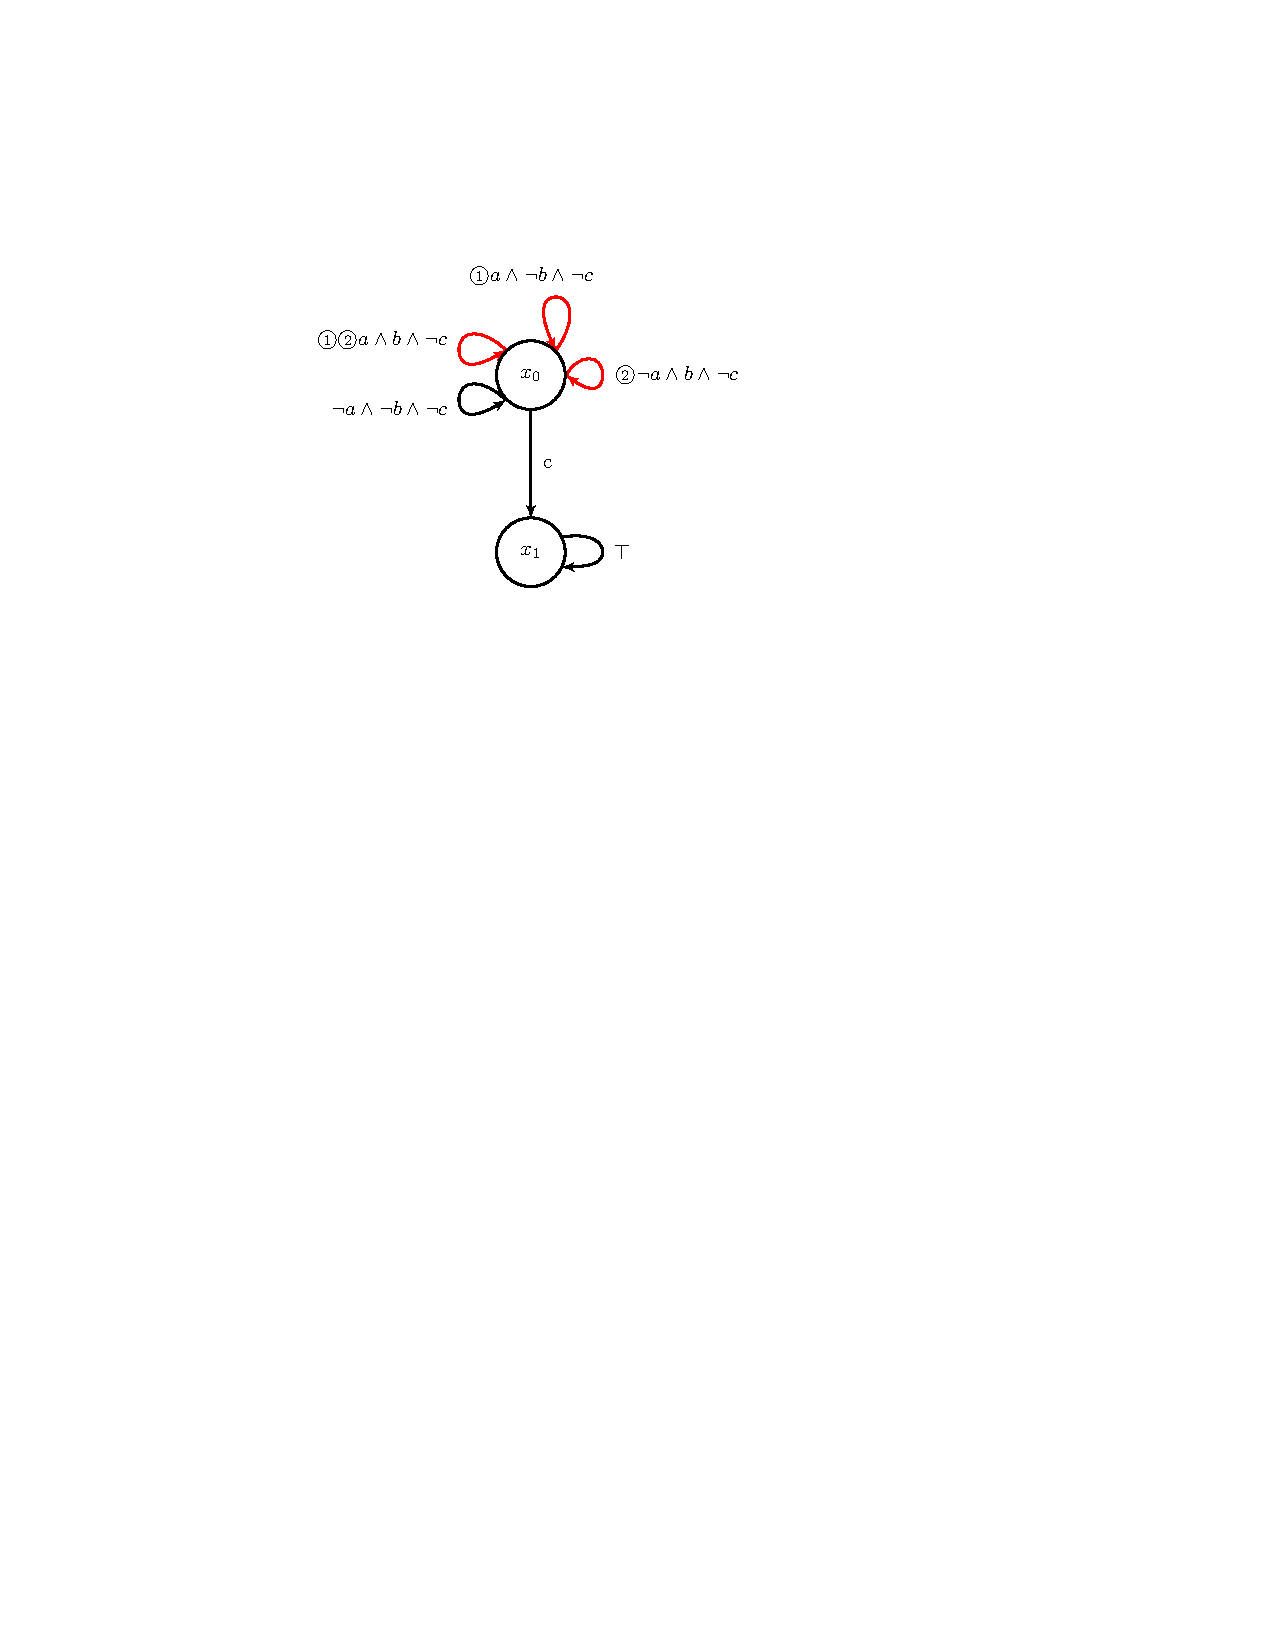
\includegraphics[bb=140 498 368 682,width=5cm]{automaton1.pdf}
   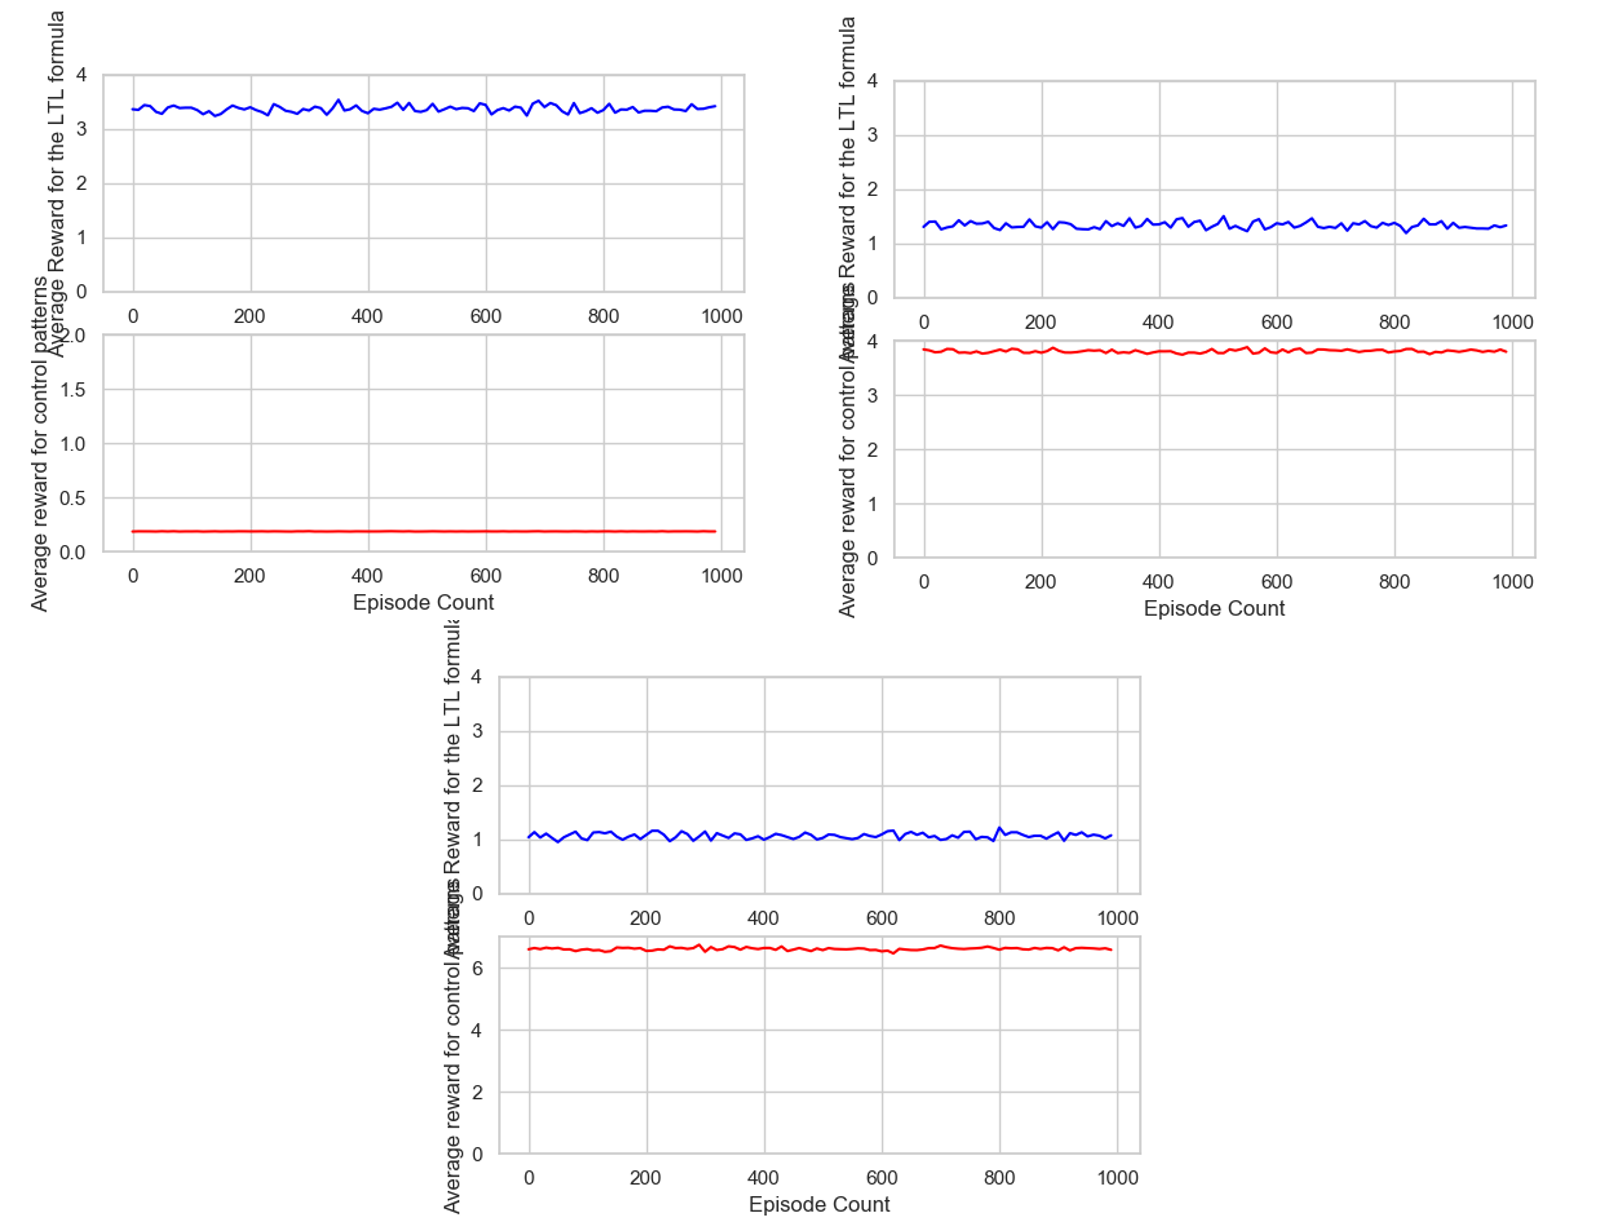
\includegraphics[width = 12cm]{simulate_TD_v_15000_5000_rn_all_rsink_1000.png}
   \caption{The average rewards of $\mathcal{R}_1$ and average rewards of $\mathcal{R}_2$ by the supervisor obtained from the learning with $r_{n} = 0.1$ (left above), $r_n = 0.7$ (right above), and $r_n = 1.2$ (below).}
   \label{sim1}
\end{figure}

\section{Conclusion}
In this chapter, we proposed a novel RL-method for the synthesis of a supervisor for an LTL specification using an augmented limit-deterministic generalized automaton. The proposed method synthesize a supervisor satisfying a given LTL specification and ensure the safety with probability 1 under the supervisor if such supervisors exist. The following arguments are future works. (i) We investigate the method synthesizing a supervisor that maximizes the satisfaction probability. (ii) We expand our proposed method to a hierarchical control. (iii) We apply our proposed method to multiagent systems.


%%%%%%%%%%%% 5th Chapter %%%%%%%%%%%%%%%%%%%%%%%%%%%%%%%%%%%%%%%%%%%%%%%%%%%
%\chapter{Conclusions}

%%%%%%%%%%%% Appendix %%%%%%%%%%%%%%%%%%%%%%%%%%%%%%%%%%%%%%%%%%%%%%%%%%%
\appendix
%%%%%%%%%%%% Appendix A %%%%%%%%%%%%%%%%%%%%%%%%%%%%%%%%%%%%%%%%%%%%%%%%%%%
\chapter{Proofs}

\begin{proof}[Proof of lemma \ref{lemma3-1}]
Suppose that $MC^{\otimes}_{\pi}$ satisfies neither conditions 1 nor 2. Then, there exist a policy $\pi$, $i \in \{ 1, \ldots ,h \}$, and $j_1$, $j_2$ $\in \{ 1, \ldots ,n \}$ such that $\delta^{\otimes i}_{\pi} \cap \bar{F}^{\otimes}_{j_1} = \emptyset$ and $\delta^{\otimes i}_{\pi} \cap \bar{F}^{\otimes}_{j_2} \neq \emptyset$. In other words, there exists a nonempty and proper subset $J \in 2^{\{ 1, \ldots ,n \}} \setminus \{ \{ 1, \ldots ,n \}, \emptyset \}$ such that $ \delta^{\otimes i}_{\pi} \cap \bar{F}^{\otimes}_j \neq \emptyset $ for any $j \in J$.
 For any transition $ (s,a,s^{\prime}) \in \delta^{\otimes i}_{\pi} \cap \bar{F}^{\otimes}_j$, the following equation holds by the properties of the recurrent states in $MC^{\otimes}_{\pi}$\cite{ESS}.
\begin{align}
  \sum_{k=0}^{\infty} p^k((s,a,s^{\prime}),(s,a,s^{\prime})) = \infty,
  \label{eq15}
\end{align}
where $p^k((s,a,s^{\prime}),(s,a,s^{ \prime}))$ is the probability that the transition $(s,a,s^{\prime})$ reoccurs after it occurs in $k$ time steps. Eq. (\ref{eq15}) means that all transition in $R^{\otimes i}_{\pi}$ occurs infinitely often. However, the memory state $v$ is never reset in $R^{\otimes i}_{\pi}$ by the assumption. This directly contradicts Eq.\ (\ref{eq15}).
\end{proof}


\begin{proof}[Proof of Theorem \ref{theorem3-1}]
  Suppose that $\pi^{\ast}$ is an optimal policy but does not satisfy the LTL formula $\varphi$. Then, for any recurrent class $R^{\otimes i}_{{\pi}^{\ast}}$ in the Markov chain $MC^{\otimes}_{{\pi}^{\ast}}$ and any accepting set $\bar{F}^{\otimes}_j$ of the product MDP $M^{\otimes}$,  $\delta^{\otimes i}_{\pi^{\ast}} \cap \bar{F}^{\otimes}_j = \emptyset$
  holds by Lemma \ref{lemma1}. Thus, the agent under the policy $\pi^{\ast}$ can obtain rewards only in the set of transient states. We consider the best scenario in the assumption. Let $p^k(s,s^{\prime})$ be the probability of going to a state $s^{\prime}$ in $k$ time steps after leaving the state $s$, and let $Post(T^{\otimes}_{\pi})$ be the set of states in recurrent classes that can be transitioned from states in $T^{\otimes}_{\pi}$ by one action. For the initial state $s_{init}$ in the set of transient states, it holds that
  \begin{align}
    V^{\pi^{\ast}}\!(s_{init})
     =\ & \sum_{k=0}^{\infty} \sum_{s \in T^{\otimes}_{\pi^{\ast}}} \gamma^k p^k(s_{init}, s)  \sum_{s^{\prime} \in T^{\otimes}_{\pi^{\ast}} \cup Post(T^{\otimes}_{\pi^{\ast}})} P^{\otimes}_{\pi^{\ast}}(s^{\prime}| s) \mathcal{R}(s, a, s^{\prime})\nonumber \\
     \leq\ & r_p \sum_{k=0}^{\infty} \sum_{s \in T^{\otimes}_{\pi^{\ast}}} \gamma^k p^k(s_{init}, s), \nonumber
  \label{eqth11}
  \end{align}
  where the action $a$ is selected by $\pi^{\ast}$. By the property of the transient states, for any state $s^{\otimes}$ in $T^{\otimes}_{\pi^{\ast}}$, there exists a bounded positive value $m$ such that $ \sum_{k=0}^{\infty} \gamma^k p^k(s_{init}, s) \leq \sum_{k=0}^{\infty} p^k(s_{init}, s) < m$ \cite{ESS}. Therefore, there exists a bounded positive value $\bar{m}$ such that $V^{\pi^{\ast}}(s_{init}) < \bar{m}$.
  Let $\bar{\pi}$ be a positional policy satisfying $\varphi$. We consider the following two cases.
  \begin{enumerate}
    \vspace{2mm}
    \item Assume that the initial state $s_{init}$ is in a recurrent class $R^{\otimes i}_{\bar{\pi}}$ for some $ i \in \{1,\ldots,h\} $.
    For any accepting set $\bar{F}^{\otimes}_j$, $\delta^{\otimes i}_{\bar{\pi}} \cap \bar{F}^{\otimes}_j \neq \emptyset$ holds by the definition of $\bar{\pi}$. The expected discounted reward for $s_{init}$ is given by
    \begin{align}
      V^{\bar{\pi}}(s_{init})
       &= \sum_{k=0}^{\infty} \sum_{s \in R^{\otimes i}_{\bar{\pi}}} \gamma^k p^k(s_{init}, s) \sum_{s^{\prime} \in R^{\otimes i}_{\bar{\pi}}}  P^{\otimes}_{\bar{\pi}}(s^{\prime}\ |\ s) \mathcal{R}(s, a, s^{\prime}), \nonumber
    \end{align}
    where the action $a$ is selected by $\bar{\pi}$. Since $s_{init}$ is in $R^{\otimes i}_{\bar{\pi}}$, there exists a positive number $\bar{k} = \min \{ k\ ;\ k \geq n, p^{k}(s_{init}, s_{init}) > 0 \}$ \cite{ESS}. We consider the worst scenario in this case. It holds that
    \begin{align}
      V^{\bar{\pi}}(s_{init})
       \geq & \sum_{k=n}^{\infty} p^{k}(s_{init}, s_{init}) \sum_{i=1}^{n} \gamma^{k-i} r_p \nonumber \\
       \geq & \sum_{k=1}^{\infty} p^{k \bar{k}}(s_{init}, s_{init}) \sum_{i=0}^{n-1} \gamma^{k \bar{k} - i} r_p \nonumber \\
       > & r_p \sum_{k=1}^{\infty} \gamma^{k \bar{k}} p^{k \bar{k}}(s_{init}, s_{init}), \nonumber
    \end{align}
whereas all states in $R(MC^{\otimes}_{\bar{\pi}})$ are positive recurrent because $|S^{\otimes}| < \infty$ \cite{ISP}. Obviously, $p^{k \bar{k}}(s_{init}, s_{init}) \geq (p^{\bar{k}}(s_{init}, s_{init}))^k > 0$ holds for any $k \in (0, \infty)$ by the Chapman-Kolmogorov equation \cite{ESS}. Furthermore, we have $\lim_{k \rightarrow \infty} p^{k \bar{k}}(s_{init}, s_{init}) > 0$ by the property of irreducibility and positive recurrence \cite{SM}. Hence, there exists $\bar{p}$ such that $0<\bar{p}<p^{k \bar{k}}(s_{init}, s_{init})$ for any $k \in (0, \infty]$ and we have
    \begin{align}
       V^{\bar{\pi}}(s_{init}) > & r_p \bar{p} \frac{\gamma^{\bar{k}}}{ 1 - \gamma^{\bar{k}} }. \nonumber
    \end{align}

    Therefore, for any $\bar{m} \in (V^{\pi^{\ast}}(s_{init}), \infty)$ and any $r_p < \infty$, there exists $\gamma^{\ast}<1$ such that $\gamma > \gamma^{\ast}$ implies $V^{\bar{\pi}}(s_{init}) > r_p \bar{p} \frac{\gamma^{\bar{k}}}{ 1 - \gamma^{\bar{k}} } > \bar{m}.$

    \item Assume that the initial state $s_{init}$ is in the set of transient states $T_{\bar{\pi}}^{\otimes}$.
    $P^{M^{\otimes}}_{\bar{\pi}}(s_{init} \models \varphi) > 0$ holds by the definition of $\bar{\pi}$. For a recurrent class $R^{\otimes i}_{\bar{\pi}}$ such that $\delta^{\otimes i}_{\bar{\pi}} \cap \bar{F}^{\otimes}_j \neq \emptyset$ for each accepting set
    $\bar{F}^{\otimes}_j$, there exist a number $\bar{l} > 0$, a state $\hat{s}$ in $Post(T^{\otimes}_{\bar{\pi}}) \cap R^{\otimes i}_{\bar{\pi}}$, and a subset of transient states $\{ s_1, \ldots , s_{\bar{l}-1} \} \subset T^\otimes_{\bar{\pi}}$ such that $p(s_{init}, s_1)>0$, $p(s_{i}, s_{i+1})>0$ for $i \in \{ 1,...,\bar{l}-2 \}$, and $p(s_{\bar{l}-1}, \hat{s})>0$ by the property of transient states.
    Hence, it holds that $p^{\bar{l}}(s_{init}, \hat{s}) > 0$ for the state $\hat{s}^{\otimes}$. Thus, by ignoring rewards in $T^{\otimes}_{\bar{\pi}}$, we have
     \begin{align}
        V^{\bar{\pi}}(s_{init}) %\nonumber \\
        \geq\ & \gamma^{\bar{l}} p^{\bar{l}}(s_{init}, \hat{s}) \sum_{k=0}^{\infty} \sum_{s^{\prime} \in R^{\otimes i}_{\bar{\pi}}} \gamma^k p^k(\hat{s}, s^{\prime}) \sum_{s^{\prime \prime} \in R^{\otimes i}_{\bar{\pi}}} P^{\otimes}_{\bar{\pi}}(s^{\prime \prime} | s^{\prime}) \mathcal{R}(s^{\prime}, a, s^{\prime \prime}) \nonumber \\
        >\ & \gamma^{\bar{l}} p^{\bar{l}}(s_{init}, \hat{s}) r_p \bar{p} \frac{\gamma^{\bar{k}^{\prime}}}{ 1 - \gamma^{\bar{k}^{\prime}} }, \nonumber
     \end{align}
     where $\bar{k}^{\prime}  \geq n$ is a constant and $0<\bar{p}< p^{k \bar{k}^{\prime}}(\hat{s}, \hat{s})$ for any $k \in (0, \infty]$.
     Therefore, for any $r_p < \infty$ and any $\bar{m} \in (V^{\pi^{\ast}}(s_{init}), \infty)$, there exists $\gamma^{\ast}<1$ such that $\gamma > \gamma^{\ast}$ implies
%     \begin{align*}
%     V^{\bar{\pi}}(s^{\otimes}_{init}) > \\P^{M^{\otimes}}_{\bar{\pi}}(s^{\otimes}_{init} \models \varphi) \gamma^{\bar{l}} p^{\bar{l}}(s^{\otimes}_{init}, \hat{s}^{\otimes}) r_p \bar{p} \gamma^{\bar{k}^{\prime}} p^{\bar{k}^{\prime}}(\hat{s}^{\otimes},\hat{s}^{\otimes}) \frac{1}{ 1 - \gamma^{\bar{k}^{\prime}} } > \bar{m}
%     \end{align*}
     $V^{\bar{\pi}}(s_{init}) > \gamma^{\bar{l}} p^{\bar{l}}(s_{init}, \hat{s}) \frac{r_p \bar{p} \gamma^{\bar{k}^{\prime}}}{ 1 - \gamma^{\bar{k}^{\prime}} } > \bar{m}$.
  \end{enumerate}

The results contradict the optimality assumption of $\pi^{\ast}$.
\end{proof}


%%%%%%%%%%%% 謝辞 %%%%%%%%%%%%%%%%%%%%%%%%%%%%%%%%%%%%%%%%%%%
\begin{acknowledgement}
	I would like to express my deep sense of gratitude to my adviser Professor
	Toshimitsu Ushio, Graduate School of Engineering Science, Osaka University,
	for his invaluable, constructive advice and constant encouragement during this work.
	Professor Ushio's deep knowledge and his eye for detail have inspired me much.
\end{acknowledgement}

%%%%%%%%%%%% References %%%%%%%%%%%%%%%%%%%%%%%%%%%%%%%%%%%%%%%%%%%%%%%%%%
%適当に変えてねー.
\begin{thebibliography}{99}
  \bibitem{BK2008}
  C.\ Baier and J.-P.\ Katoen,
  \textit{Principles of Model Checking}.
  MIT Press, 2008.
  \bibitem{Clarke2018}
  E.\ M.\ Clarke, Jr., O.\ Grumberg, D.\ Kroening, D.\ Peled, and H.\ Veith,
  \textit{Model Checking}, 2nd Edition.
  MIT Press, 2018.
  \bibitem{KB2008}
  M.\ Kloetzer, C.\ Belta,
  ``A fully automated framework for control of linear systems from temporal logic specifications,''
  \textit{IEEE Trans.\ Autom.\ Contr.}, vol.\ 53, no.\ 1, pp.\ 287--297, 2008.
  \bibitem{Gazit2009}
  H.\ Kress-Gazit, G.\ E.\ Fainekos, and G.\ J.\ Pappas,
  ``Temporal-logic-based reactive mission and motion planning,''
  \textit{IEEE Trans.\ Robotics}, vol.\ 25, no.\ 6, pp.\ 1370--1381, 2009.
  \bibitem{WTM2012a}
  T.\ Wongpiromsarn, U.\ Topcu, and R.\ M.\ Murray,
  ``Receding horizon temporal logic planning,''
  \textit{IEEE Trans.\ Autom.\ Contr.}, vol.\ 57, no.\ 11, pp.\ 2817--2830, 2012.
  \bibitem{SU2018}
  A.\ Sakakibara and T.\ Ushio,
  ``Decentralized supervision and coordination of concurrent discrete event systems under LTL constraints,''
   in \textit{Proc.\ 14th International Workshop on Discrete Event Systems}, 2018, pp.\ 18-23.
  \bibitem{Belta2017}
  C.\ Belta, B.\ Yordanov, and E.\ A.\ Gol,
  \textit{Formal Methods for Discrete-Time Dynamical Systems}.
  Springer, 2017.
  \bibitem{Puterman}
  M.\ L.\ Puterman,
  \textit{Markov Decison Processes, Discrete Stochastic Dynamic Programming}.
  John Wiley \& Sons, Inc., 1994.

  \bibitem{WTM2012}
  E.\ M.\ Wolff, U.\ Topcu, and R.\ M.\ Murray,
  ``Robust control of uncertain Markov decision processes with temporal logic specifications,''
  in \textit{Proc.\ 51st IEEE Conference on Decision and Control}, 2012, pp.\ 3372--3379.
  \bibitem{Sadigh2014}
  D.\ Sadigh, E.\ S.\ Kim, A.\ Coogan, S.\ S.\ Sastry, and S.\ Seshia,
  ``A learning based approach to control synthesis of Markov decision processes for linear temporal logic specifications,''
  \textit{in Proc.\ 53rd IEEE Conference on Decision and Control}, pp.\ 1091-1096, 2014.
  \bibitem{Sutton}
  R.\ S.\ Sutton and A.\ G.\ Barto,
  \textit{Reinforcement Learning: An Introduction}, 2nd Edition.
  MIT Press, 2018.
  \bibitem{HU2015}
  M.\ Hiromoto and T.\ Ushio,
  ``Learning an optimal control policy for a Markov decision process under linear temporal logic specifications,''
  in \textit{Proc.\ 2015 IEEE Symposium on Adaptive Dynamic Programming and Reinforcement Learning}, 2015, pp.\ 548-555.
  \bibitem{SEJK2016}
  S.\ Sickert, J.\ Esparaza, S.\ Jaax, and J.\ K\v{r}et\`{i}nsk\'{y},
  ``Limit-deterministic B\"{u}chi automata for linear temporal logic,''
   in \textit{International Conference on Computer Aided Verification}, 2016, pp.\ 312-332.
  \bibitem{HAK2019}
  M.\ Hasanbeig, A.\ Abate, and D.\ Kroening,
  ``Logically-constrained reinforcement learning,'' \textit{arXiv:1801.08099v8}, Feb.\ 2019.
  \bibitem{Hahn2019}
  E.\ M.\ Hahn, M.\ Perez, S.\ Schewe, F.\ Somenzi, A.\ Triverdi, and D.\ Wojtczak,
  ``Omega-regular objective in model-free reinforcement learning,''
  \textit{Lecture Notes in Computer Science}, no.\ 11427, pp.\ 395--412, 2019.
  \bibitem{HKAKPL2019}
  M.\ Hasanbeig, Y.\ Kantaros, A.\ Abate, D.\ Kroening, G.\ J.\ Pappas, and I.\ Lee,
  ``Reinforcement learning for temporal logic control synthesis with probabilistic satisfaction guarantee,''
  \textit{arXiv:1909.05304v1}, 2019.
  \bibitem{BWZP2019}
  A.\ K.\ Bozkurt, Y.\ Wang, M.\ Zavlanos, and M.\ Pajic,
  ``Control synthesis from linear temporal logic specifications using model-free reinforcement learning,''
  \textit{arXiv:1909.07299}, 2019.
  \bibitem{ESS}
  R.\ Durrett,
  \textit{Essentials of Stochastic Processes}, 2nd Edition. ser. Springer texts in statistics. New York; London; Springer, 2012.
  \bibitem{ISP}
  L.\ Breuer,
  ``Introduction to Stochastic Processes'', [Online]. Available: https://www.kent.ac.uk/smsas/personal/lb209/files/sp07.pdf
  \bibitem{SM}
  S.M.\ Ross,
  \textit{Stochastic Processes}, 2nd Edition. University of California, Wiley, 1995.
  \bibitem{Singh1998}
  S. Singh, T. Jaakkola, M. L. Littman, and C. Szepes\'{v}ari,
  ``Convergence results for single-step on-policy reinforcement learning algorithms'' \textit{Machine Learning},
  vol.~38, no.~3, pp,~287--308, 1998.
  \bibitem{Owl}
  J.~Kretínsk\'{y}, T.~Meggendorfer, S.~Sickert, ``Owl: A library for $\omega$-words, automata,
  and LTL,'' in \textit{Proc.~16th International Symposium on Automated Technology for Verification and Analysis}, 2018,  pp.~543–550.
  %https://doi.org/10.1007/978-3-030-01090-4\_34
\end{thebibliography}
%\bibliographystyle{myjunsrt}
%\bibliography{refs}

\end{document}
